\documentclass[11pt]{article}
\usepackage[utf8]{inputenc}


\usepackage{url}
\usepackage{breakurl}
\usepackage[breaklinks]{hyperref}
\usepackage[super]{nth}
\usepackage{bm}
\usepackage{booktabs}
\usepackage{enumerate}
\usepackage{graphicx}
\usepackage{multirow}
\usepackage{multicol}
\usepackage{amsmath}
\usepackage{amstext}
\usepackage{amssymb}
\usepackage{pdflscape}
\usepackage{multirow}
\usepackage{amsfonts}
\usepackage{rotating}
\usepackage{xcolor}
\usepackage{placeins}
\usepackage{amssymb}
\usepackage{listings}
\usepackage{xcolor}
\usepackage{adjustbox}
\usepackage{tabularx}
\usepackage{booktabs,csvsimple}
\usepackage[font=scriptsize]{caption} 


\definecolor{codegreen}{rgb}{0,0.6,0}
\definecolor{codegray}{rgb}{0.5,0.5,0.5}
\definecolor{codepurple}{rgb}{0.58,0,0.82}
\definecolor{backcolour}{rgb}{0.95,0.95,0.92}

\lstdefinestyle{mystyle}{
    backgroundcolor=\color{backcolour},   
    commentstyle=\color{codegreen},
    keywordstyle=\color{magenta},
    numberstyle=\tiny\color{codegray},
    stringstyle=\color{codepurple},
    basicstyle=\ttfamily\footnotesize,
    breakatwhitespace=false,         
    breaklines=true,                 
    captionpos=b,                    
    keepspaces=true,                 
    numbers=left,                    
    numbersep=5pt,                  
    showspaces=false,                
    showstringspaces=false,
    showtabs=false,                  
    tabsize=2
}

\lstset{style=mystyle}
%\usepackage{algpseudocode}
\usepackage{natbib}
\usepackage{setspace} 
\usepackage{latexsym}
\usepackage{subfig}
\allowdisplaybreaks
\usepackage{array}
%\usepackage{subcaption}
\newcolumntype{H}{>{\setbox0=\hbox\bgroup}c<{\egroup}@{}}
\usepackage{pdfpages}
\usepackage{diagbox}
\usepackage{graphicx}
\usepackage{soul}

\usepackage{capt-of}% or \usepackage{caption}
\usepackage{varwidth}
\newsavebox\tmpbox

\usepackage{csvsimple,booktabs}
\usepackage{filecontents}

\usepackage{afterpage}
\graphicspath{{Images/}}

\linespread{1.5}
%%\singlespacing 

\usepackage{geometry}
\geometry{
	a4paper,
	total={160mm,220mm},
	left=16mm,
	top=22mm,
	bottom=30mm,
}

\usepackage[linesnumbered,ruled,vlined]{algorithm2e, algorithmic}

% Keywords command
\providecommand{\keywords}[1]
{
  \small	
  \textbf{\textit{Keywords---}} #1
}

\title{Campaign Optimization in Telecommunication with Communication Limitations\\}
\author{Dursun Koc $^{a}$ \\ 
	dursun.koc@turkcell.com.tr, \\\\
	Dilek Gunnec $^{a}$ $^{\ast}$\\ 
	dilek.gunnec@ozyegin.edu.tr, ORCID ID: 0000-0002-0749-2584 \\\\
$^{a}$ Ozyegin University, Department of Industrial Engineering, Istanbul, Turkey \\ 
$^{\ast}$ Corresponding author \\ }
	
\date{}

\begin{document}
\maketitle
\begin{abstract}
For marketers, the main objective is to introduce their companies products or services to their customers or potential customers. Most of the studies, prior to this study, were on how to find the right audience for a marketing campaign. However, after finding the right target audience for a campaign, planing the communication to the target audience is also an important task. Such a plan should be fine-tuned not to irritate customers by sending too many messages, considering the communication channels' capacities, and it should also be compliant with the governments' regulations on marketing activities as well. In this study we propose a mathematical model which considers various communication limitations, and communication channels' capacities. In order to solve such a problem we propose a basic greedy heuristic, and a linear programming relaxation heuristic; later, we improved the greedy heuristic by implementing a small-scale linear programming model for finding a rough estimation for the expected number of communication for each campaign.\end{abstract}\hspace{10pt}

\keywords{Campaign Optimization, Telecommunication Networks, Greedy Heuristic.}

\newpage

\section{Introduction}

There are two main strategies marketers use to introduce their products or services to existing or potential customers; inbound and outbound marketing strategies. In inbound marketing the communication is started by the customer (by entering a store, visiting a website, etc.), and s/he is presented with offers at the first opportunity during this interaction. On the other hand, in outbound marketing, a target audience (e.g., people of ages between 20 and 30, and living in New York City) is selected and contacted via channels such as a call-center, or by sending SMSs or making IVR calls. Thus, the process of reaching to the customer can be designed by the marketer. However, this may lead it being seen as interruptive and the target audience can easily find a way to dismiss the message. This makes it inefficient for the company as there is cost associated with reaching the customers through marketing activities. For example, sending SMS messages to a customer who is unlikely to respond is a loss, but, not sending it at all is also a loss from revenue \citep{sarkar}.  

%When a customer visits any of the inbound channels, e.g., a web-page, and the customer fulfills the rules, the message is given to the customer, so inbound marketing is also considered as content marketing. The marketer creates content and tries to gain customer interest using social media. 

%On the other hand, outbound marketing strategy depends on mass media tools to push the message about a product or a service. Outbound marketing is mostly seen as interruptive and the target audience can easily find a way to dismiss the message. From a companies’ perspective it can be very inefficient; because sending a message to a customer who is unlikely to respond has a cost; moreover, not sending the message to a customer who is more likely to respond is a loss from revenue \citep{sarkar}. 

Marketers have to wisely identify the right target audience because one of the keys to a good relationship with customers is keeping your offers relevant to the customers’ need \citep{malthouse}. A mismatch can cause a negative perception for the brand, and further lead the customer to block all communication channels.  In addition to identifying the right target audience, the most appropriate communication channel and the right time should also be determined.

%so the company will lose its chance to make a relevant or profitable communication opportunity in the future. In outbound campaigns the marketer tries to reach customers on her own initiative without customers' direct request; however in inbound campaigns a customer has a request and the marketer tries to direct that demand in line with her own goals. At this point, outbound campaigns are difficult to work with, but they can be effective for demand generation. 

Large amount of customer data is needed, for effective outbound marketing. Therefore companies collect more information about their customers, which causes information asymmetry \citep{waerdt}. As the governments are responsible for protecting their citizens’ rights, they make laws and regulations on this information asymmetry. (e.g., The General Data Protection Regulation (GDPR) law in EU). According to such regulations, a customer can request the company to stop processing its data.

In this respect, deciding who should receive a specific offer is one of the essential questions in outbound marketing. In addition to identifying the right target audience, the most appropriate communication channel and the right time should also be determined.

To avoid such customer response, companies need to apply some limitation on outbound communication to their customers. Outbound marketing campaigns need to be well planned with regard to time, target audience, channel and content. In this study, we optimize outbound campaigns regarding time and channel while keeping communication under certain limitations. Such limitations can either be a result of legislation or a result of marketing strategy not to irritate customers.

The remaining of this paper is structured as follows. In \S \ref{s:literature-review}, we review the related literature. In \S \ref{s:problem-model}, we describe the problem in detail and present our mathematical model for the problem. In \S \ref{s:solution-method}, we explain our proposed solution methods. In \S \ref{s:num-analysis}, we present our computational results. Finally, we conclude in \S \ref{s:conclusion}.

%%%%%%%%%%%%%%%%%%%%%%%%%%%%%%%%%%%%%%%%%%%%%%%%%%%%%%%%%%
%%%%%%%%%%%%%%%%%%%%%%%%%%%%%%%%%%%%%%%%%%%%%%%%%%%%%%%%%%

\section{Literature Review}  \label{s:literature-review}

In the industry, outbound campaigns are mostly designed regarding the target audience. Machine learning methods, statistics and business rules and regulations are used to find the right target audience, and the message about the product is sent to customers; moreover database marketing community also tries to estimate the expected value of an offer to a specific customer from a specific channel \citep{cohen_exp, oliveira_hypr}. In direct marketing, marketers select a portion of the customer group with the highest probability of expecting the offer, and then add them to their target audience for the marketing campaign \citep{owczarczuk}. However, even if the offer addresses the customer’s need, most of the time customer can dismiss the message because of the wrong channel or because of the wrong time. Having the right channel and the right time with the right audience is the most desired case, but it is not free. The cost of some channels can be high while some others are cheaper. Further, with social network effects some of the targeting can become unnecessary and costly.\\

In today’s world, marketers have multiple channels to introduce their product or services, and many studies have shown the importance of omni-channel sales strategies \citep{shankar, park}. In the essence customers want to interact with the company via multiple channels, companies’ challenge is to provide a nearly identical environment for each channel \citep{bell}. Customer can get information about a product or service from one channel, but the purchase can be from another channel \citep{park}. Even the information about the product or service can be solidified by a series of messages from different channels. At this point it is crucial to employ additional constraints regarding multiple channels when optimizing the campaign.\\

Most of the studies about campaign optimization focus on obtaining the right target audience for the campaign \citep{goul}; however, they usually ignore campaign channels, or optimize the online campaigns. They are finding the best matched campaign for a given online search only, or web-page banner optimization \citep{liu}, and the success criteria or the objective function for such models is often the click through rate or the action rate. Such objective functions do not truly represent the advertisers’ benefit and rather focus on the publishers’ benefit \citep{altshuler}. Our model will be directly related to the advertisers’ benefit.\\

Different studies work on different industries and various business constraints; but the mathematical models mostly seems similar, and can be counted as assignment problem, or more specifically multi-dimensional knapsack problem \citep{cohen_exp, oliveira_hypr}. For solving ILP (Integer Linear Programming), MIP(Mixed Integer Programming) models, numerous methods and tools have been introduced\citep{fallah_bb, chu_mip}, however due to the complexity of the problem, handling big models remains a technical difficulty. Although the branch and bound (B\&B) algorithm has been presented as the definitive and deterministic solution, when the number of variables and the number of constraints get larger, the B\&B algorithm does not provide a solution in reasonable time \citep{herrera_pbb, sato}. Because of that reason some work on parallel B\&B algorithm\citep{fallah_bb, sato}; but computational resources required to run the algorithm increases.\\ \citeauthor{cohen_exp} applied a greedy approach to a similar problem \citep{cohen_exp}. Multidimensional knapsack problems having multiple resource constraints with binary decision variables, which is similar to our model have been dealt with greedy-like heuristic methods \citep{akcay_mdkp}.

Although studies related to campaign management are common in marketing, there is increasing interest to this area from operations research and computer science areas, as the abundant data require complex data analysis skills. In my thesis, after such data analysis, we plan to introduce optimization methods which are not yet commonly used to tackle such problems. Specifically, one of our main contributions will be utilizing from network optimization tools to produce high quality solutions.\\

In this study, we plan to develop a model which tries to maximize the number of interactions for the campaigns decided by marketing team, while not exceeding the communication limitations. In the second place, we also try to increase the number of interaction to the most influential customers. We believe that influential customers can spread our message to a broader audience. In order to find the influential customer we will use customers' call and product purchase data.

\section{Campaign Optimization Problem}  \label{s:problem-model}

In this section, we describe the problem in detail and propose a mathematical model which maximizes the number of prioritized campaigns presented to customers while adhering to the communication limitations required by the company.

%(\S \ref{s:problem-math}). 

%\subsection{Problem Description} \label{s:problem-desc}

A telecommunication company in Turkey, provides different tariffs, products and services to its customers. In order to introduce them to its existing and potential customers, marketing teams launch daily and weekly campaigns. A campaign is a marketing activity that offers benefits, such as free usage or lower prices, to a predefined customer group. The customers are contacted via a set of communication channels for a specific period of time. Despite being presented with benefits, customers may find this process annoying for many reasons, e.g., products/services may not be appealing to them or the timing/method of communication may be a problem. Thus, before launching a campaign, marketers analyze customer data to determine the right target group. Then, they follow a set of rules before reaching out to / communicating with the customers.

The frequency of contacting a customer (i.e., sending a message over one of the communication channels) is one of such rules. It is hold below a certain level so that customers are not disturbed frequently. The number of messages sent to a customer in one day, or the number of customers a campaign can be presented to are limited as well. Each communication channel has a capacity of usage for each day. Each campaign has a different priority and belongs to different quota categories. Our objective is to maximize the number of communications of the highest priority campaigns while abiding by the above rules.  

%Campaigns are categorized in two dimensions; the first dimension is quota categories which describes filters for a campaign and the second one is priority categories which describes the importance of a campaign. Each campaign belongs to a quota category and each quota category has a limitation on the number of messages sent to a customer, both in a daily, and a weekly basis; 

%moreover each campaign has a limitation unique to its own; and finally, each communication channel has a capacity that should not be exceeded for each day. Each campaign is bound to a priority category.\\

%We study Turkcell’s outbound campaign management, and use an initial model to maximize the number of campaigns while abiding the rules for reaching to customers.

We use a mathematical model to solve this problem where decisions are given weekly and a rolling horizon approach is used for limitations on the number of times a customer is contacted. Next, we present our mathematical model. 


%\subsection{Mathematical Model} \label{s:problem-math}

%In this section, we present an integer programming model for the campaign optimization problem described at \S \ref{s:problem-desc}. We first introduce the notation and then present the model.\\


\begin{singlespace}
% General Math Model
\noindent \textbf{Sets}\\

\noindent ${\mathcal{C}}$: Set of campaigns \\
\noindent ${\mathcal{U}}$: Set of customers \\
\noindent ${\mathcal{H}}$: Set of communication channels \\
\noindent ${\mathcal{D}}$: Set of days (7 days of a week) \\
\noindent ${\mathcal{I}}$: Set of quota categories \\
\noindent ${\mathcal{P}}$: Set of priority categories \\


\noindent \textbf{Decision Variables}\\

\noindent $X_{{c}{u}{h}{d}}=1$, if a message on campaign $c \in \mathcal{C}$ will be sent to customer $u \in \mathcal{U}$ through channel $h \in \mathcal{H}$ on day $d \in \mathcal{D}$, and 0 otherwise.\\

\noindent \textbf{Parameters}\\

\noindent (Note that ``communication limit'' represents the maximum number of times a customer can be contacted via communication channels.) \\

\noindent $e_{{c}{u}}=1$, if customer $u \in \mathcal{U}$ is eligible for campaign $c \in \mathcal{C}$, and 0 otherwise.\\

\noindent $s_{{c}{u}{h}{d}}=1$, if customer $u \in \mathcal{U}$ is contacted about campaign $c \in \mathcal{C}$, through channel $h \in \mathcal{H}$, on day $d \in \mathcal{D}$ the previous week and 0 otherwise.\\

\noindent $q_{{i}{c}}=1$, if campaign $c \in \mathcal{C}$ is in quota category $i \in \mathcal{I}$, and 0 otherwise.\\

\noindent $r_{{c}{p}}$ priority value of campaign $c \in \mathcal{C}$ regarding priority type $p \in \mathcal{P}$.\\

\noindent $b$ communication limit per customer for the planning horizon.\\

\noindent $k$ communication limit per customer for each day.\\

\noindent $l_{c}$ communication limit per customer for campaign $c \in \mathcal{C}$.\\

\noindent $m_{i}$ communication limit for quota category $i \in \mathcal{I}$ for the planning horizon.\\

\noindent $n_{i}$ communication limit for quota category $i \in \mathcal{I}$ for each day.\\

\noindent $t_{{h}{d}}$ capacity for channel $h \in \mathcal{H}$ on day $d \in \mathcal{D}$.\\

\noindent The mathematical formulation for this campaign optimization problem is presented next.
\end{singlespace}
\vspace{-0.5cm}
\begin{align}
\text{IP: }\text{Maximize} & \displaystyle
\sum\limits_{p\in \mathcal{P}}
\sum\limits_{c\in \mathcal{C}}
\sum\limits_{u\in \mathcal{U}}
\sum\limits_{h\in \mathcal{H}}
\sum\limits_{d\in \mathcal{D}}
X_{{c}{u}{h}{d}}  r_{{c}{p}} \label{mathmodel_obj}&
\\
\text{subject to} \notag\\
&X_{{c}{u}{h}{d}} \leq e_{{c}{u}}&\forall c \in \mathcal{C}, \forall u \in \mathcal{U}, \forall h \in \mathcal{H}, \forall d \in \mathcal{D}, \label{mathmodel_eligibility}&\\
&\sum\limits_{h\in\mathcal{H}}X_{{c}{u}{h}{d}} \leq 1 &\forall c \in \mathcal{C}, \forall u \in \mathcal{U}, \forall d \in \mathcal{D}, \label{mathmodel_singlechannel}&\\
&\sum\limits_{h\in\mathcal{H}}\sum\limits_{c\in\mathcal{C}}\sum\limits_{d\in\mathcal{D}}X_{{c}{u}{h}{d}} \leq b &\forall u \in \mathcal{U}, \label{mathmodel_percustomercommlimit}&\\
&\sum\limits_{h\in\mathcal{H}}\sum\limits_{c\in\mathcal{C}}X_{{c}{u}{h}{d}} \leq k &\forall u \in \mathcal{U}, \forall d \in \mathcal{D}, \label{mathmodel_percustomercommlimit_day}&\\
&\sum\limits_{d\in\mathcal{D}}\sum\limits_{h\in\mathcal{H}}X_{{c}{u}{h}{d}} \leq l_{c} &\forall c \in \mathcal{C}, \forall u \in \mathcal{U}, \label{mathmodel_percustomercamplimit}&\\
&\sum\limits_{d\in\mathcal{D}}\sum\limits_{h\in\mathcal{H}}\sum\limits_{c\in\mathcal{C}}X_{{c}{u}{h}{d}}  q_{{i}{c}} \leq m_{i} &\forall u \in \mathcal{U}, \forall i \in \mathcal{I}, \label{mathmodel_weeklyquotalimit}&\\
&\sum\limits_{h\in\mathcal{H}}\sum\limits_{c\in\mathcal{C}}X_{{c}{u}{h}{d}}  q_{{i}{c}} \leq n_{i} &\forall u \in \mathcal{U}, \forall d \in \mathcal{D}, \forall i \in \mathcal{I}, \label{mathmodel_dailyquotalimit}&\\
&\sum\limits_{u\in\mathcal{U}}\sum\limits_{c\in\mathcal{C}}X_{{c}{u}{h}{d}} \leq t_{{h}{d}} &\forall d \in \mathcal{D}, \forall h \in \mathcal{H}, \label{mathmodel_channellimit}&\\
&\sum\limits_{h\in\mathcal{H}}\sum\limits_{c\in\mathcal{C}}q_{{i}{c}}\left(\sum_{d=1}^{w}X_{{c}{u}{h}{d}} + \sum_{d=w+1}^{7}s_{{c}{u}{h}{d}}\right) \leq m_{i} &\forall u \in \mathcal{U}, \forall i \in \mathcal{I}, \forall w \in [1,6], \label{mathmodel_weeklyquotalimit_rh}&\\
&\sum\limits_{h\in\mathcal{H}}\sum\limits_{c\in\mathcal{C}}\left(\sum_{d=1}^{w}X_{{c}{u}{h}{d}} + \sum_{d=w+1}^{7}s_{{c}{u}{h}{d}}\right) \leq b &\forall u \in \mathcal{U}, \forall w \in [1,6], \label{mathmodel_percustomercommlimit_rh}&\\
&\sum\limits_{h\in\mathcal{H}}\left( \sum_{d=1}^{w}X_{{c}{u}{h}{d}} + \sum_{d=w+1}^{7}s_{{c}{u}{h}{d}}\right) \leq l_{c} &\forall c \in \mathcal{C}, \forall u \in \mathcal{U}, \forall w \in [1,6], \label{mathmodel_percustomercamplimit_rh}&\\
&X_{{c}{u}{h}{d}} \in \{0,1\}&\forall c \in \mathcal{C}, \forall u \in \mathcal{U}, \forall h \in \mathcal{H}, \forall d \in \mathcal{D}, \label{mathmodel_integrity}
\end{align}\\

The objective function \eqref{mathmodel_obj} maximizes the prioritized campaign communication. Constraints \eqref{mathmodel_eligibility} ensure that only eligible customers are contacted for each campaign. Constraints \eqref{mathmodel_singlechannel} say that a customer should not be targeted for the same campaign from different channels a day. Constraints \eqref{mathmodel_percustomercommlimit} limit the total number of times a customer can be contacted in a week, and constraints \eqref{mathmodel_percustomercommlimit_rh} consider the previous week and make sure it is taken into account when calculating the limits, i.e., uses a rolling horizon. Constraints \eqref{mathmodel_percustomercommlimit_day} define an upper-bound for the total number of contacts made to each customer in a single day. Constraints \eqref{mathmodel_percustomercamplimit} define an upper-bound for total number of communication to each customer per campaign for the whole period; and constraints \eqref{mathmodel_percustomercamplimit_rh} extend the upper-bound for total number of communication to each customer per campaign regarding the previous period. Campaigns are grouped by their marketing purpose, and for each of these groups we have combined limitations. Constraints \eqref{mathmodel_weeklyquotalimit} draw a limitation on the number of communications about campaigns that fell in specific groups. $q_{{i}{c}}$ equals to 1 if the campaign $c$ is in category  $i$. Likewise, constraints \eqref{mathmodel_weeklyquotalimit_rh} limit the number of communications for campaign quota categories regarding previous period. Constraints \eqref{mathmodel_dailyquotalimit} ensure that the number of communications for campaign quota categories for each day is not exceeded. Constraint \eqref{mathmodel_channellimit} ensures that each communication channels' capacity are not exceeded; and finally constraint \eqref{mathmodel_integrity} ensures that the variable $X_{{c}{u}{h}{d}}$ is either 0 or 1.\\

Due to its complexity, large instances of this problem may not be solved by using exact methods as quickly as required in practice. Thus, we develop a heuristic approach that can attain high-quality solutions within reasonable time.

%%%%%%%%%%%%%%%%%%%%%%%%%%%%%%%%%%%%%%%%%%%%%%%%%%%%%%%%%%
%%%%%%%%%%%%%%%%%%%%%%%%%%%%%%%%%%%%%%%%%%%%%%%%%%%%%%%%%%

\section{Solution Methods}  \label{s:solution-method}

In this section, we describe three heuristics. The first two are based on a greedy approach, and the last one is based on a linear programming relaxation. In \S \ref{s:greedy_heuristic_basic} we implement a basic greedy heuristic which considers only the campaign priorities, and in \S \ref{s:greedy_heuristic_improved} we improve it to consider the number of eligible people in addition to campaign priorities, and finally in \S \ref{s:lp_relaxation_heuristic} we solve the mathematical model by LP-Relaxation by defining the  $X_{{c}{u}{h}{d}}$ variables as real numbers between 0 and 1.

\subsection{Basic Greedy Heuristic} \label{s:greedy_heuristic_basic}

We use the following greedy algorithm (Algorithm 1) to solve the campaign optimization problem described in \ref{s:problem-model}. We assign  the most important campaign (the one with the highest priority) first. We do not apply any specific ranking for days, channels and customers. For feasibility check, we consider only the constraints in which $X_{{c}{u}{h}{d}}$ variables are contained.

More specifically, Algorithm 1 starts by sorting campaigns with respect to their $r_{cp}$ values, and starting from the campaign with the highest value, sets the corresponding campaign value for $X_{cuhd}$ to 1. Then, checks the feasibility for constraints \eqref{mathmodel_eligibility} to \eqref{mathmodel_integrity} using the $CheckFeasibility$ function, which takes the indices of the variable $X_{cuhd}$ being modified and $X$ variable set, and it finds out the constraint functions which contains the $X_{cuhd}$ variable, and checks their value per modification.
\\

\begin{algorithm}[H]
\DontPrintSemicolon
\KwIn{Constraints\eqref{mathmodel_eligibility} to \eqref{mathmodel_integrity}}
\KwOut{$X_{{c}{u}{h}{d}}$, $c\in\mathcal{C}$, $u\in\mathcal{U}$, $h\in\mathcal{H}$, $d\in\mathcal{D}$ }
  \SetKwFunction{FSortCampaigns}{SortCampaigns}
%  \SetKwFunction{FCheckFeasibility}{CheckFeasibility}

%  \SetKwProg{Fn}{Function}{:}{}
%   \Fn{\FCheckFeasibility{$X$, $c$, $u$, $h$, $d$}}{
%         FunctionsToCheck = $IPFeasibilityFunctions$ containig $X_{{c}{u}{h}{d}}$\;
%         satisfied = FunctionsToCheck(X)\;
%         \KwRet satisfied\;
%   }\;
Sort campaigns (c \in C) \; $such that$ \; ($r_{c_{1}p} \geq r_{c_{2}p}$)\\
\For{$c \gets 1$ \textbf{to} $C$}{
    \For{$d \gets 1$ \textbf{to} $D$}{
        \For{$h \gets 1$ \textbf{to} $H$}{
            \For{$u \gets 1$ \textbf{to} $U$}{
                 $X_{cuhd}$ = 1\;
                 \If {any one of the constraints (2) to (13) are violated} {
                    $X_{cuhd}$ = 0\;
                 }
            }
        }
    }
}
\Return{$X_{{c}{u}{h}{d}}$}\;
\caption{Basic Greedy Heuristic}
\label{algo:greedy_impl1}
\end{algorithm}

\subsection{Improved Greedy Heuristic} \label{s:greedy_heuristic_improved}
In this section, we improve the basic greedy heuristic using a new linear programming model. In this model, we take into account the possible number of eligible people that can be reached for each campaign. This way, we create a new method to prioritize the campaigns. 
% In order to find better solution, we improved our understanding of prior campaigns by implementing a linear programming model of the problem. 
% \subsubsection{The New LP model} \label{s:problem-math-lp}
%Prioritizing campaigns with respect to In this model, instead of assigning specific customers to specific campaigns, we . 
%BURDA KALDIM
Depending on the constraints campaigns with higher priority can have smaller audience, likewise campaigns with lesser priority can have much greater audience. As our objective function \eqref{mathmodel_obj} is product of both campaign priority and total number of messages sent, our greedy algorithm should start with the campaign which has higher priority and higher total number of messages to be sent. Let say if campaign-1 has a priority of 100 and can be sent to 1 customer, and campaign-2 has a priority of 50 and can be sent to 5 customers, then starting from campaign-2 instead of campaign-1 will result in a better solution.
\\
We first introduce the notation and then present the mathematical model for the LP. Note that the following model does not consider the individual limitations introduced in the problem definition described at section \s\ref{s:problem-model}, unlikely the model below is finding the maximum number of messages that can be sent by not caring how many messages an individual receives.\\


\noindent \textbf{New Decision Variable}\\

\noindent $Y_{{c}{d}}$, total number of messages sent about campaign $c \in \mathcal{C}$ at day $d \in \mathcal{D}$.
($\forall c \in \mathcal{C}$, $\forall d \in \mathcal{D}$ )\\
\\

\noindent \textbf{New Parameter}\\

\noindent $e_{c}$, number of customers eligible, can be calculated as $\sum\limits_{u\in\mathcal{U}}e_{{c}{u}}$ for campaign $c \in \mathcal{C}$\\

\noindent The formulation for the campaign optimization is presented next.

\begin{align}
\text{LP: }\text{Maximize} & \displaystyle
\sum\limits_{c\in \mathcal{C}}
\sum\limits_{d\in \mathcal{D}}
Y_{{c}{d}} \label{mathmodel2_obj}&
\\
\text{subject to} \notag\\
&\sum\limits_{d\in\mathcal{D}}Y_{{c}{d}} \leq l_{c}  e_{c} &&&\forall c \in \mathcal{C}, \label{mathmodel2_campaignlimit}&\\
&\sum\limits_{c\in\mathcal{C}}\sum\limits_{d\in\mathcal{D}} q_{{i}{c}} Y_{{c}{d}}\leq \sum\limits_{c\in\mathcal{C}}q_{{i}{c}} e_{c}  m_{i} &&&\forall i \in \mathcal{I}, \label{mathmodel2_weeklyquotalimit}&\\
&\sum\limits_{c\in\mathcal{C}}q_{{i}{c}} Y_{{c}{d}} \leq \sum\limits_{c\in\mathcal{C}}q_{{i}{c}} e_{c} n_{i} &&&\forall d \in \mathcal{D}, \forall i \in \mathcal{I}, \label{mathmodel2_dailyquotalimit}&\\
&\sum\limits_{c\in\mathcal{C}}\sum\limits_{d\in\mathcal{D}}Y_{{c}{d}} \leq \sum\limits_{c\in\mathcal{C}}e_{c}  b, \label{mathmodel2_weeklylimit}&\\
&\sum\limits_{c\in\mathcal{C}}Y_{{c}{d}} \leq \sum\limits_{c\in\mathcal{C}}e_{c} k &&&\forall d \in \mathcal{D},\label{mathmodel2_dailylimit}&\\
&Y_{{c}{d}} \geq 0&&&\forall c \in \mathcal{C}, \forall d \in \mathcal{D}, \label{mathmodel2_positive}
\end{align}\\

The objective function \eqref{mathmodel2_obj} maximizes the total number of people reached over total time. Constraints \eqref{mathmodel2_campaignlimit} ensure that the number of communication for each campaign can not exceed the number of eligible customers for the campaign regarding the campaign limit, just like the constraints \eqref{mathmodel_percustomercamplimit} in the IP model. Constraints \eqref{mathmodel2_weeklyquotalimit} draw a limitation on the number of communications about campaigns that fell in specific groups for the whole period, like the constraints \eqref{mathmodel_weeklyquotalimit} in the IP model. Likewise constraints \eqref{mathmodel2_dailyquotalimit} draw a limitation on the number of communications about campaigns that fell in specific groups for a specific day which maps to \eqref{mathmodel_dailyquotalimit}. Constraints \eqref{mathmodel2_weeklylimit} and \eqref{mathmodel2_dailylimit} ensure that the number of communications in total are not exceeded weekly and daily limits both of which are shadows of the constraints \eqref{mathmodel_percustomercommlimit}, and \eqref{mathmodel_percustomercommlimit_day} respectively in the IP model; and finally constraint \eqref{mathmodel2_positive} ensure that the variable $Y_{{c}{d}}$ is a positive number.\\

The preceding mathematical model is used for finding a rough estimation for the expected number of communication for each campaign. In Algorithm \ref{algo:greedy2} (\textit{Improved Greedy Heuristic}) expected number of communication for each campaign $Y_{{c}{d}}$ is used to sort campaigns in addition to campaign priority $r_{{c}{p}}$.
\\
\\
\begin{algorithm}[H]
\DontPrintSemicolon
\KwIn{X, $c\in\mathcal{C}$, $u\in\mathcal{U}$, $h\in\mathcal{H}$, $d\in\mathcal{D}$, $IPFeasibilityFunctions$ (constraints\eqref{mathmodel_eligibility} to \eqref{mathmodel_integrity})}
\KwOut{$X_{{c}{u}{h}{d}}$, $c\in\mathcal{C}$, $u\in\mathcal{U}$, $h\in\mathcal{H}$, $d\in\mathcal{D}$ such that constraints\eqref{mathmodel_eligibility} to \eqref{mathmodel_integrity} are satisfied}
\SetKwFunction{FSortCampaigns}{SortCampaigns}
\SetKwFunction{FCheckFeasibility}{CheckFeasibility}
  \SetKwProg{Fn}{Funtion}{:}{}
  \Fn{\FCheckFeasibility{$X$, $c$, $u$, $h$, $d$}}{
        FunctionsToCheck = $IPFeasibilityFunctions$ containig $X_{{c}{u}{h}{d}}$\;
        satisfied = FunctionsToCheck(X)\;
        \KwRet satisfied\;
  }\;

$Y_{{c}{d}}$ = Solve LP Model \eqref{mathmodel2_obj} to \eqref{mathmodel2_positive}

\For{$d \gets 1$ \textbf{to} $D$}{
SortCampaigns(C) \tcp*{such that($Y_{{c_{1}}{d}}  r_{c_{1}p} \geq Y_{{c_{2}}{d}}  r_{c_{2}p}$)}
    \For{$c \gets 1$ \textbf{to} $C$}{
        \For{$h \gets 1$ \textbf{to} $H$}{
%        Order and reindex customers $u\in\mathcal{U}$ so that $\sum\limits_{c\in\mathcal{C}}\sum\limits_{h\in\mathcal{H}}\sum\limits_{d\in\mathcal{D}}X_{{c}{u_{1}}{h}{d}} \leq \sum\limits_{c\in\mathcal{C}}\sum\limits_{h\in\mathcal{H}}\sum\limits_{d\in\mathcal{D}}X_{{c}{u_{2}}{h}{d}}$
            \For{$u \gets 1$ \textbf{to} $U$}{
                 $X_{cuhd}$ = 1\;
                 \If {\textbf{not} CheckFeasibility(X,c,u,h,d)} {
                    $X_{cuhd}$ = 0\;
                 }
            }
        }
    }
}
\Return{$X$}
\caption{Greedy Heuristic improved by LP}
\label{algo:greedy2}
\end{algorithm}

\subsection{LP-relaxation} \label{s:lp_relaxation_heuristic}
In this section, we relax the model described at \S \ref{s:problem-model} to a linear programming model by setting \eqref{mathmodel_integrity} to $X_{{c}{u}{h}{d}} \in [0,1],\forall c \in \mathcal{C}, \forall u \in \mathcal{U}, \forall h \in \mathcal{H}, \forall d \in \mathcal{D}$. After that we apply Algorithm \ref{algo:lprelax} (\textit{LP-Relaxation with Greedy Approach}) to find a solution.\\
\begin{algorithm}[H]
\DontPrintSemicolon
\KwIn{X, $c\in\mathcal{C}$, $u\in\mathcal{U}$, $h\in\mathcal{H}$, $d\in\mathcal{D}$, $IPFeasibilityFunctions$ (constraints\eqref{mathmodel_eligibility} to \eqref{mathmodel_integrity})}
\KwOut{$X_{{c}{u}{h}{d}}$, $c\in\mathcal{C}$, $u\in\mathcal{U}$, $h\in\mathcal{H}$, $d\in\mathcal{D}$ such that constraints\eqref{mathmodel_eligibility} to \eqref{mathmodel_integrity} are satisfied}
  \SetKwFunction{FSortCampaigns}{SortCampaigns}
  \SetKwFunction{FCheckFeasibility}{CheckFeasibility}

  \SetKwProg{Fn}{Funtion}{:}{}
  \Fn{\FCheckFeasibility{$X$, $c$, $u$, $h$, $d$}}{
        FunctionsToCheck = $IPFeasibilityFunctions$ containig $X_{{c}{u}{h}{d}}$\;
        satisfied = FunctionsToCheck(X)\;
        \KwRet satisfied\;
  }\;
$X_{{c}{u}{h}{d}}$ = Solve LP Model \eqref{mathmodel_obj} to\eqref{mathmodel_integrity}

\For{$d \gets 1$ \textbf{to} $D$}{
SortCampaigns(C) \tcp*{such that $r_{c_{1}p} \geq r_{c_{2}p}$}
    \For{$c \gets 1$ \textbf{to} $C$}{
        \For{$h \gets 1$ \textbf{to} $H$}{
            \For{$u \gets 1$ \textbf{to} $U$}{
                 \If{$X_{cuhd}>0$ and $X_{cuhd}<1$}{
                 $X_{cuhd}$ = 1\;
                 \If {\textbf{not} CheckFeasibility(X,c,u,h,d)} {
                    $X_{cuhd}$ = 0\;
                 }
                 }
            }
        }
    }
}
\Return{$X$}\;
\caption{LP-Relaxation With Greedy Approach for Campaign Optimization}
\label{algo:lprelax}
\end{algorithm}

\newpage
\section{Computational Study} \label{s:num-analysis}

In this section, we present the results of our computational study proposed. We first describe our test instances and then evaluate the performance of our proposed heuristics. All computations were performed on a computer with 64-bit Windows 10 operating system with Intel(R) Core(TM) i7-3630QM CPU 16 GB RAM, and CPLEX 20.1 was used in Python to solve campaign optimization for exact results. Heuristic algorithms are also coded in Python.

Campaigns are planned in a weekly basis. The company launches on average about 10 campaigns for around 500.000 customers through 3 channels each day. Number of quota categories is fixed to 3, but priority categories can be variable around 10.

%%%%%%%%%%%%%%%%%%%%%%%%%%%%%%%%%%%%%%%%%%%%%%%%%%%%%%%%%%
\subsection{Test Instances} \label{test_cases}
Table \ref{table:tbl_test_instances} gives a summary of the test instances we used to test our algorithms described in \S \ref{s:solution-method}. Instances from 1 to 15 can be regarded as small-sized problems, instances from 15 to 30 can be seen as medium-sized problems, instances from 30 to 45 can be seen as large-sized problems. The major player in increasing the difficulty of the problem is the customer size. A real world scenario can be similar to instances 39 to 45. We have conducted two types of tests, first we executed test instances with rich channel capacities, which looses constraint \eqref{mathmodel_channellimit}; later we cut down the channel capacity such that some of the communication possibilities are blocked by it. It should be noted that in a real world scenario, channel capacities are rich, as the company is a Telco. Parameters for each test instances can be found at appendix-\ref{s:apendix-parameters-in-test-instances} for rich channel capacity, and at appendix-\ref{s:apendix-parameters-strict-in-test-instances}.\\

\begin{table}[htb!]
\resizebox{0.65\textwidth}{!}{\begin{minipage}{\textwidth}
    \centering
    \caption[Short Caption for LoT]{Test instances for campaign optimization problem}\label{table:tbl_test_instances}
\csvautobooktabular{test_instances.csv}
\end{minipage} }
\end{table}
\clearpage

\subsection{Heuristic Performances} \label{s:test_evaluation}
First, we executed instances with rich channel capacity. We find exact solutions for instances from 1 to 17 using CPLEX MIP solver, later as the channel capacity is loose, we solved instances from 18 to 45 by solving sub-problems with grouping customers. Later we executed instances with limited channel capacity, again we find exact solutions for instances from 1 to 17 using the solver, but for instances from 18 to 45 solving sub-problems does not provide a solution rather it provides an upper bound for the solutions. Instances larger than 17 could not be solved by the solver on our test computer, so we solve those problems by solving sub problems divided by customer groups to find out an upper bound.

For rich channel capacity, we solved problems also with basic greedy heuristic described at \S \ref{s:greedy_heuristic_basic}, with improved greedy heuristic described at\S \ref{s:greedy_heuristic_improved}, and finally with LP relaxation heuristic described at \S \ref{s:lp_relaxation_heuristic}.\\

Table-\ref{table:tbl_exact_rich_results} shows each algorithms objective value gap to the exact solutions beside with the execution times in seconds for the rich channel capacity. Figure-\ref{fig:fig_durations_exact_rich} shows duration in seconds for each methods, and test instances, and Figure-\ref{fig:fig_value_gap_exact_rich} shows objective value of basic greedy, improved greedy and LP-relaxation heuristics are differ from the exact solution's objective value for the rich channel capacity. It can be inferred that the Improved Greedy algorithm can find good enough solutions with better performance in case of rich channel capacity. 
Table-\ref{table:tbl_exact_limited_results} shows each algorithms objective value gap to the exact solutions beside with the execution times in seconds for the limited channel capacity. Figure-\ref{fig:fig_durations_exact_limited_17} shows duration in seconds for each methods, and test instances, and Figure-\ref{fig:fig_value_gap_exact_limited_17} shows objective value of basic greedy, improved greedy and LP-relaxation heuristics are differ from the exact solution's objective value for the limited channel capacity. Table-\ref{table:tbl_ub_limited_results} shows objective value of basic greedy and improved greedy are differ from the upper-bound for instances from 18 to 45, and their execution time in seconds in case of limited channel capacity. The objective value of improved greedy is significantly better than the objective value of basic greedy while the exection time of both algorithm does not diverges. However the gap on the objective value of limited channel capacity case is not as tight as in the case of rich channel capacity.
The differences are calculated using the formulation described at \equationautorefname \eqref{exact_distance_formulation}.\\

        \begin{table}[htb!]
        \caption{Objective Value Gap\% and Execution Time in seconds for Rich Channel Capacity.}\label{table:tbl_exact_rich_results}
        \begin{adjustbox}{max width=1\textwidth}
        \csvautobooktabular[table head={\toprule  
           &\multicolumn{3}{c|}{Objective Value Gap} & \multicolumn{4}{c}{Execution Time in seconds} \\
        \cmidrule{2-4} \cmidrule{5-8} \csvlinetotablerow\\\midrule}]{n_test_results_all_exact_rich.csv}
        \end{adjustbox}
        \label{tab:test}
        \end{table}

        \begin{figure}[htb!]
        \centering
        \begin{minipage}{.6\textwidth}
            \centering
            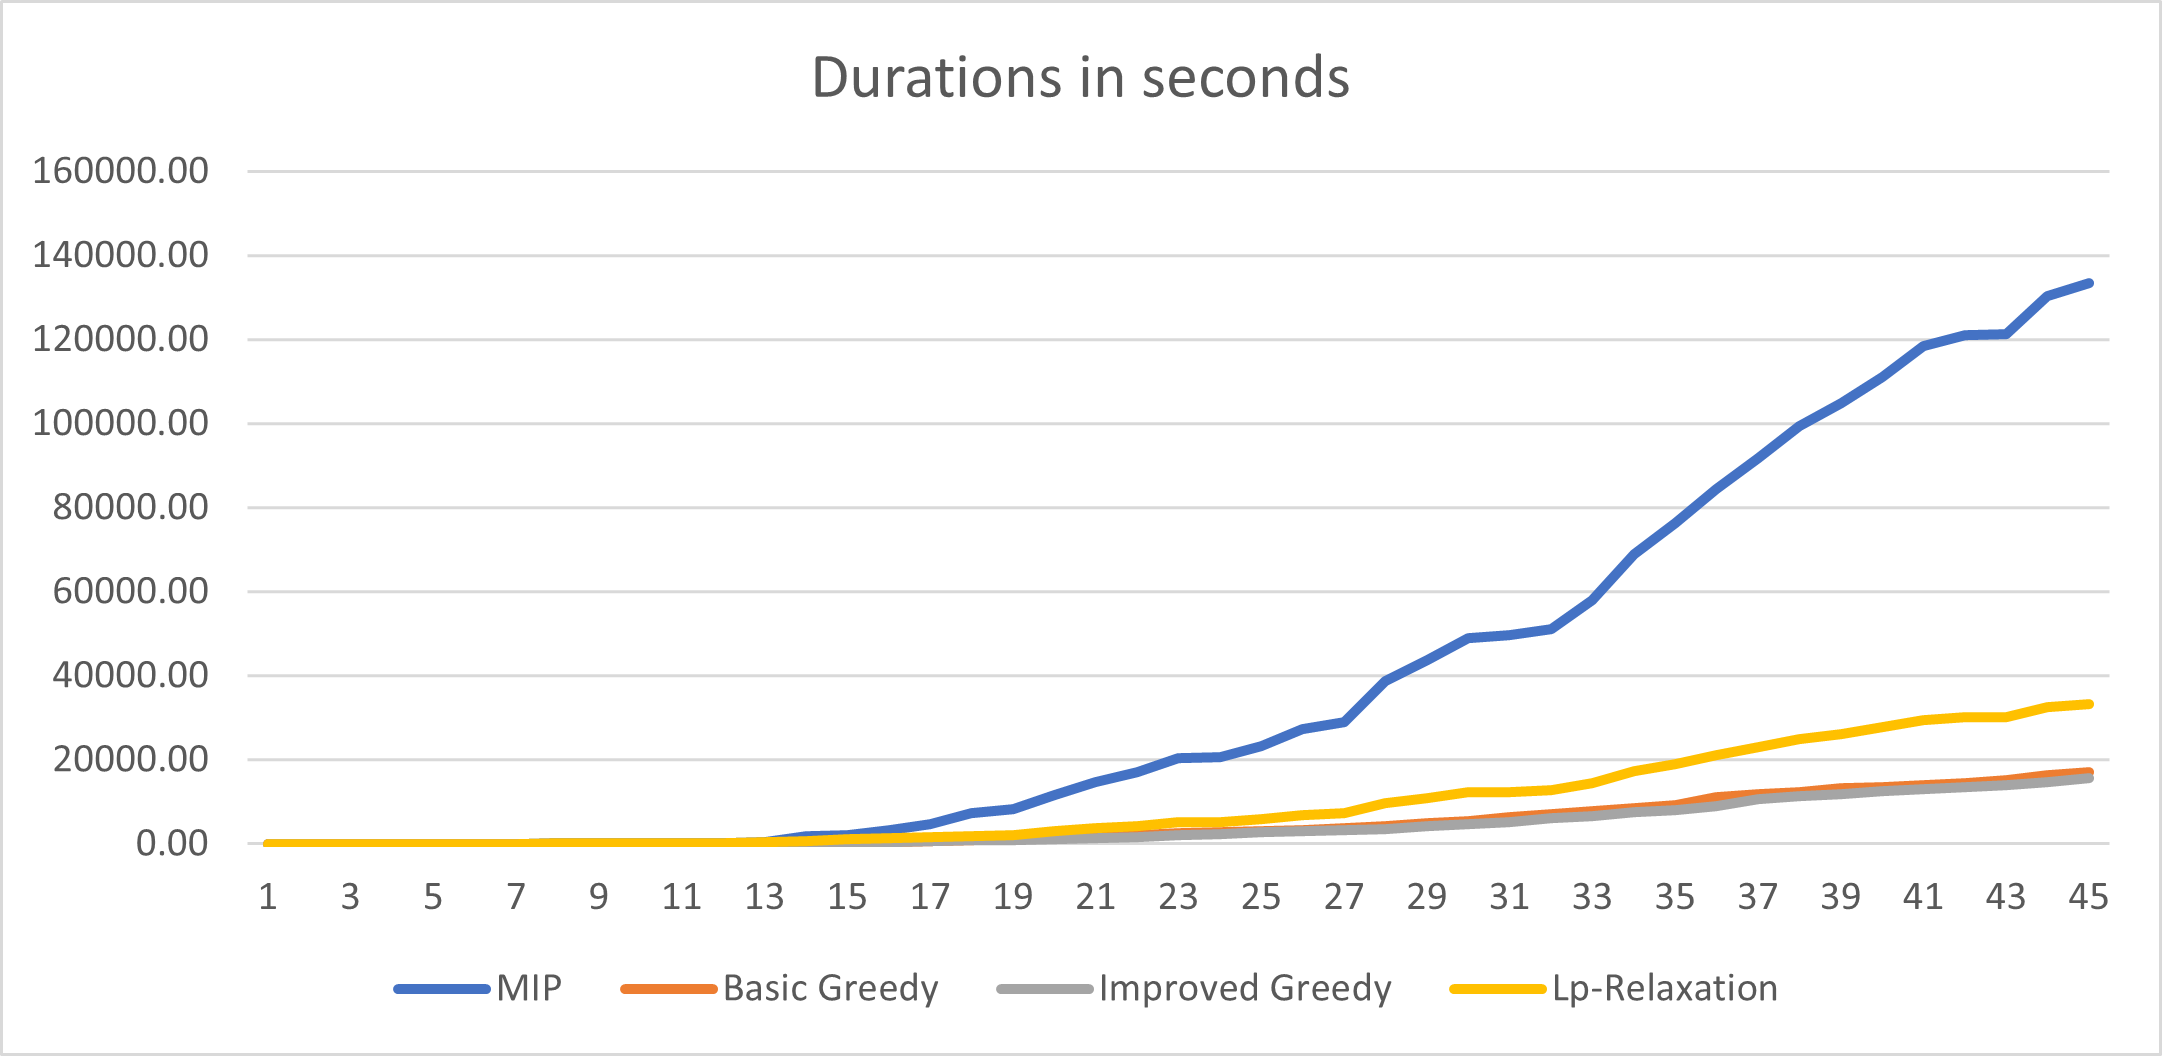
\includegraphics[width=.7\linewidth]{durations_exact_rich.png}
            \caption{Execution time in secs for Rich Channel Capacity}
            \label{fig:fig_durations_exact_rich}
        \end{minipage}%
        \begin{minipage}{.6\textwidth}
            \centering
            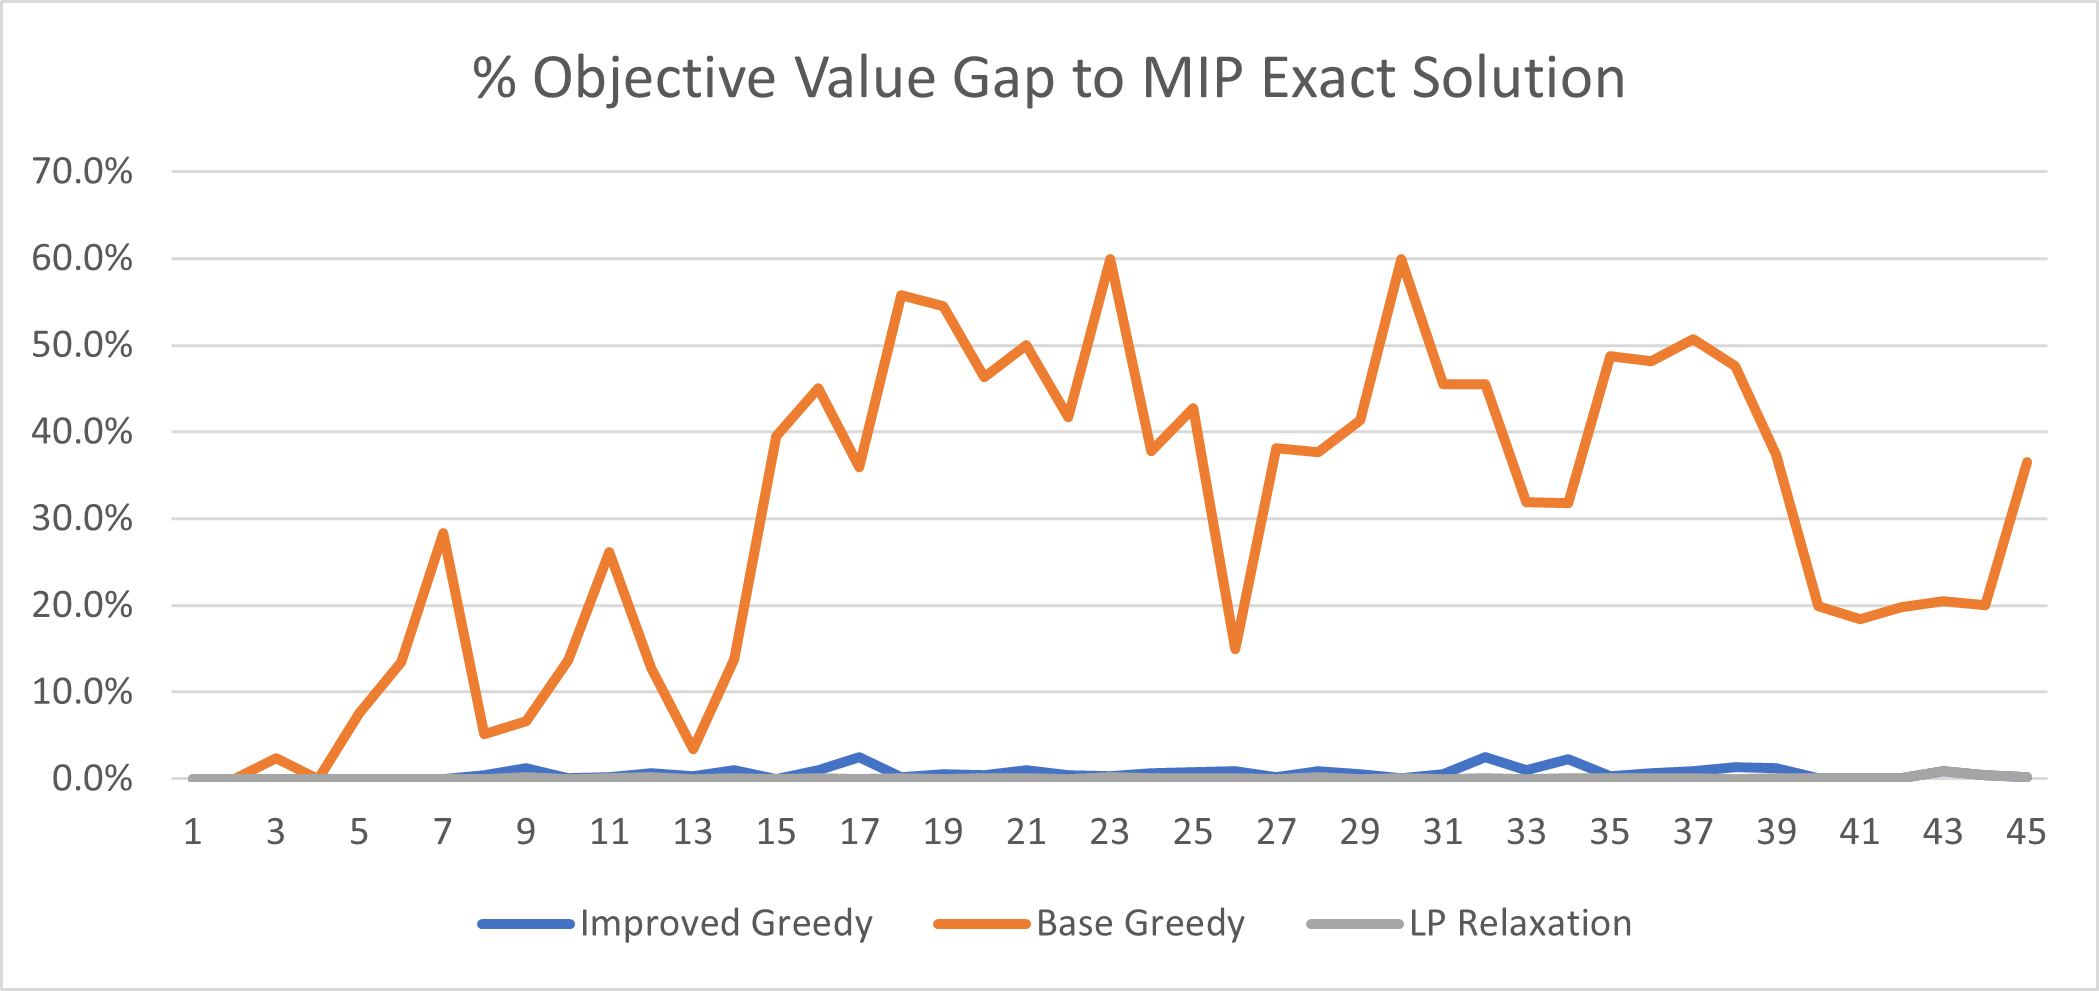
\includegraphics[width=.7\linewidth]{performance_exact_rich.png}
            \caption{\% Objective Value Gap to MIP Exact Solution for Rich Channel Capacity}
            \label{fig:fig_value_gap_exact_rich}
        \end{minipage}
        \end{figure}
        
        \begin{table}[htb!]
        \caption{Objective Value Gap\% and Execution Time in seconds for Limited Channel Capacity.}\label{table:tbl_exact_limited_results}
        \begin{adjustbox}{max width=1\textwidth}
        \csvautobooktabular[table head={\toprule  
           &\multicolumn{3}{c|}{Objective Value Gap} & \multicolumn{4}{c}{Execution Time in seconds} \\
        \cmidrule{2-4} \cmidrule{5-8} \csvlinetotablerow\\\midrule}]{n_test_results_17_exact_limited.csv}
        \end{adjustbox}
        \label{tab:test}
        \end{table}

        \begin{figure}[htb!]
        \centering
        \begin{minipage}{.6\textwidth}
            \centering
            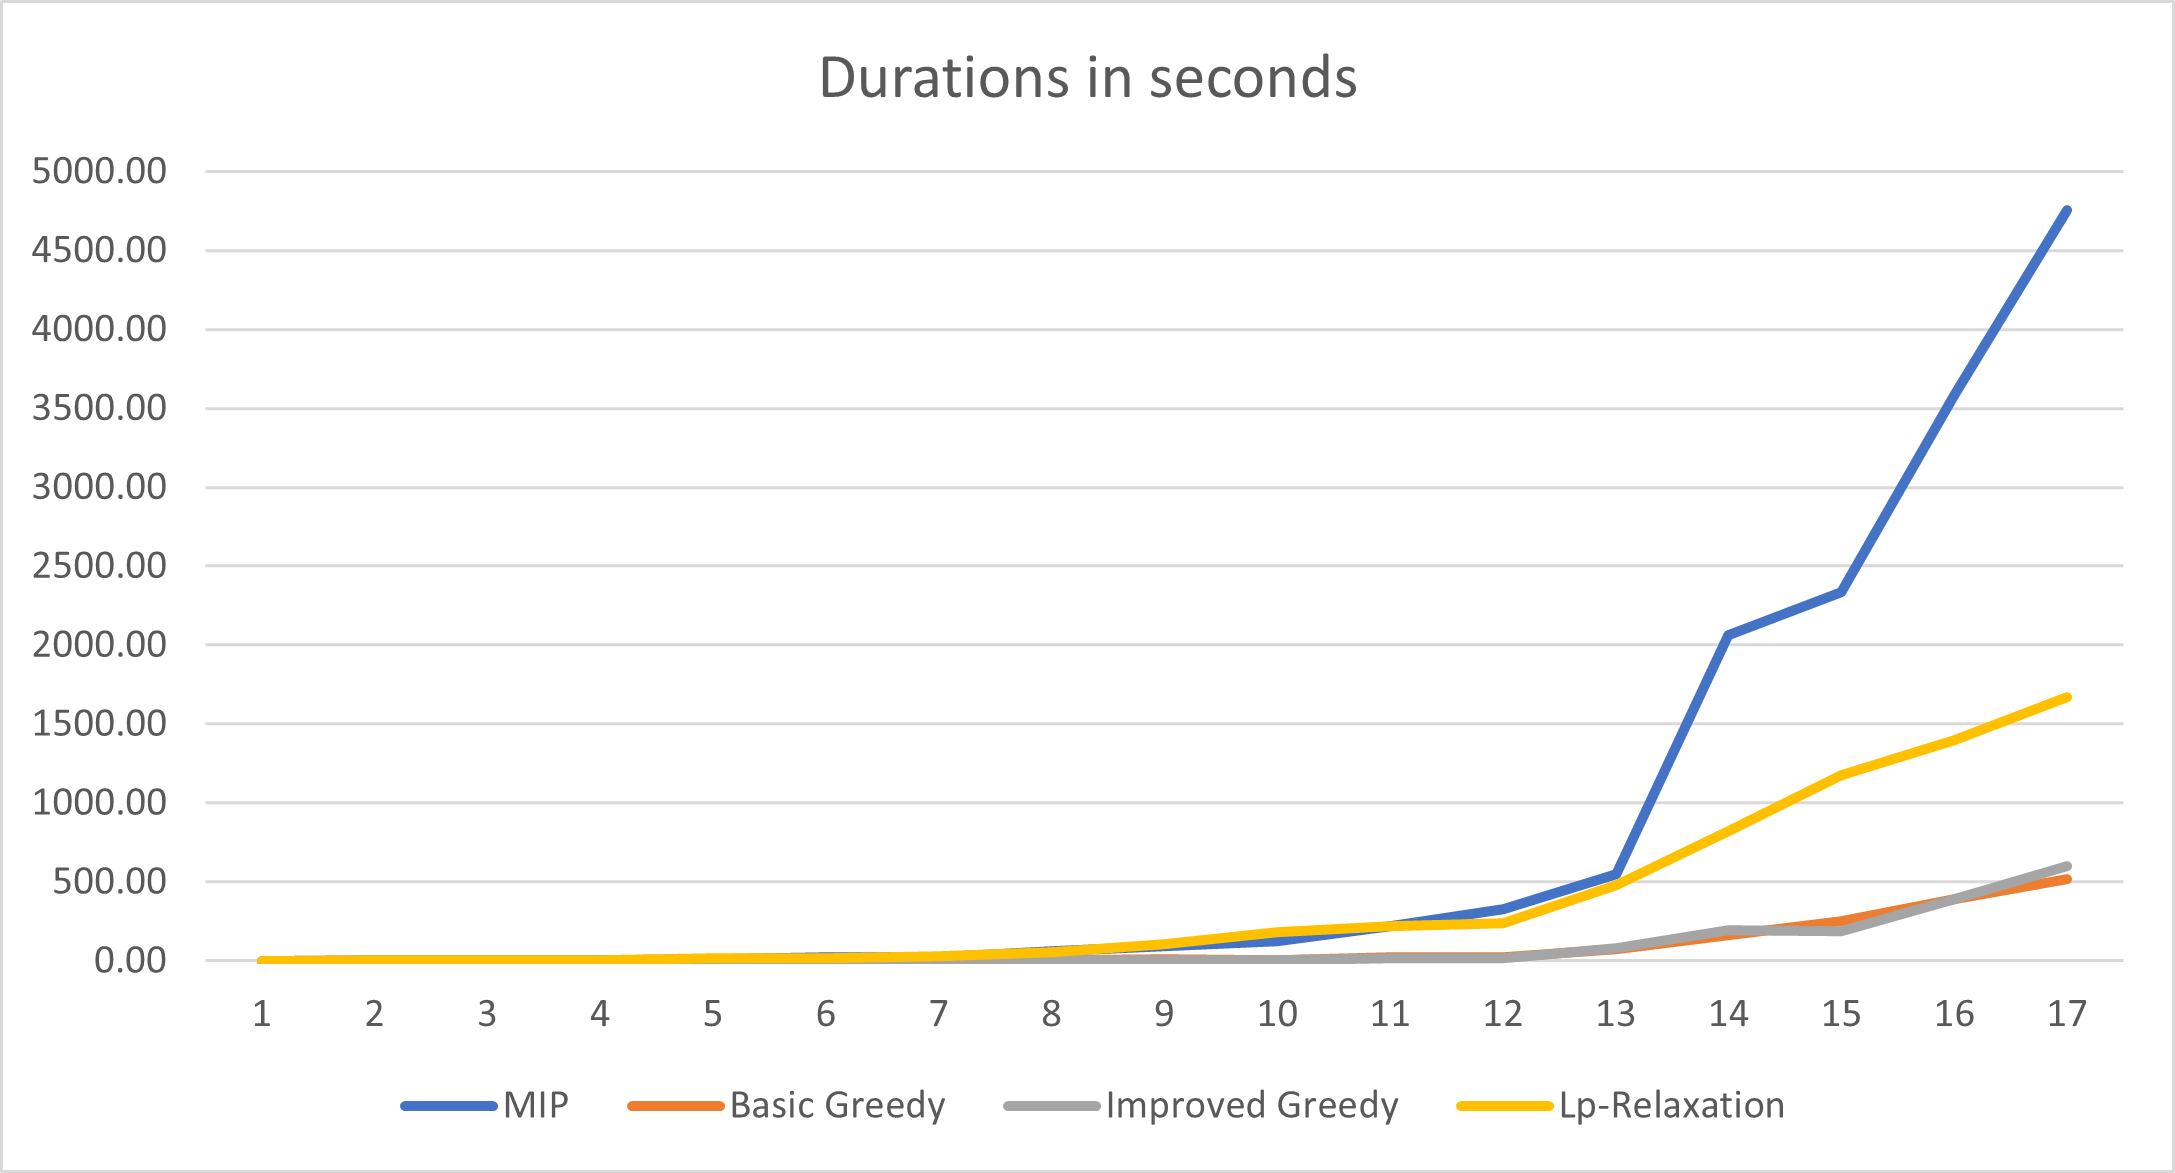
\includegraphics[width=.7\linewidth]{durations_exact_limited_17.png}
            \caption{Execution time in secs for Limited Channel Capacity}
            \label{fig:fig_durations_exact_limited_17}
        \end{minipage}%
        \begin{minipage}{.6\textwidth}
            \centering
            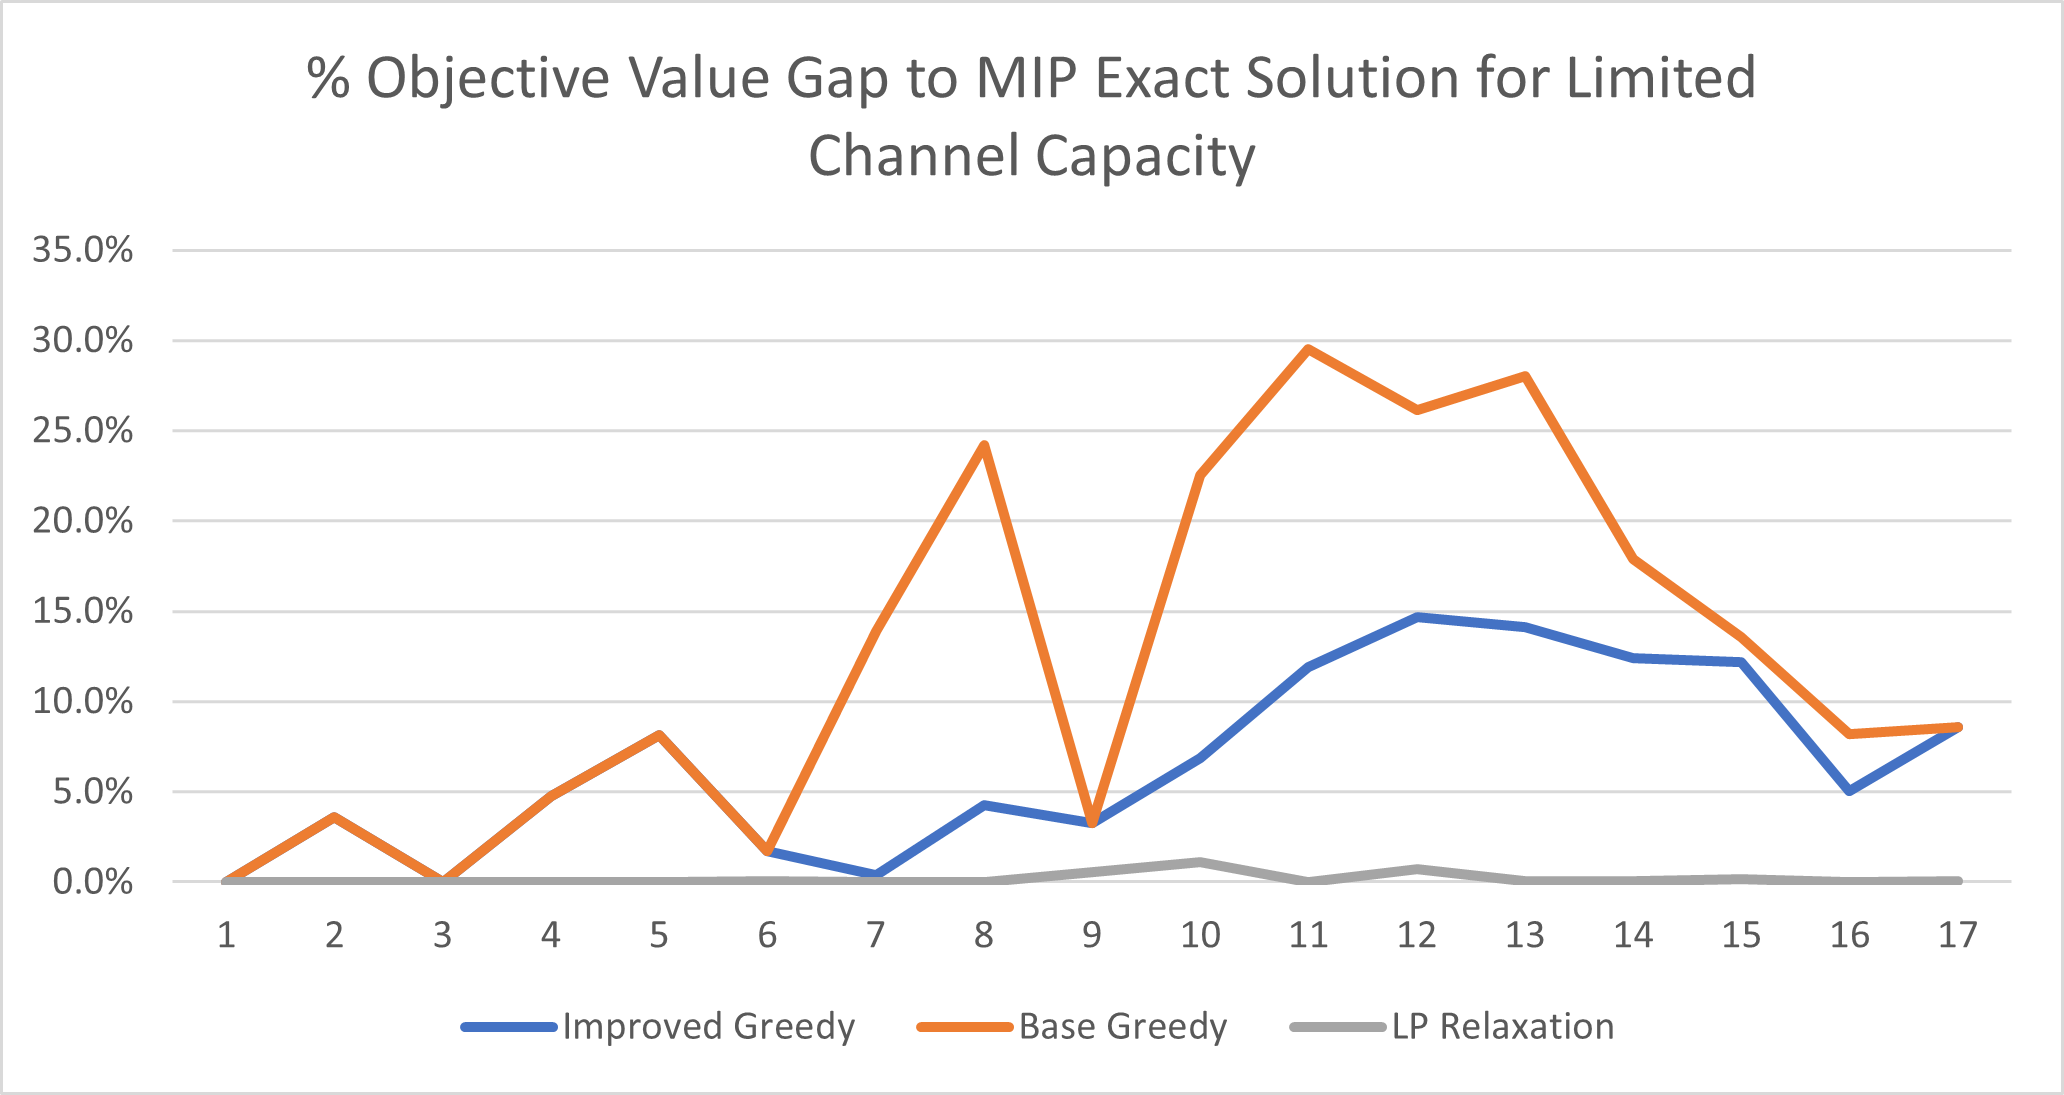
\includegraphics[width=.7\linewidth]{performance_exact_limited_17.png}
            \caption{\% Objective Value Gap to MIP Exact Solution for Limited Channel Capacity}
            \label{fig:fig_value_gap_exact_limited_17}
        \end{minipage}
        \end{figure}


        \begin{table}[htb!]
        \caption{Objective Value Gap\% to Upper-Bound and Execution Time in seconds for Limited Channel Capacity.}\label{table:tbl_ub_limited_results}
        \begin{adjustbox}{max width=1\textwidth}
        \csvautobooktabular[table head={\toprule  
           &\multicolumn{2}{c|}{Objective Value Gap} & \multicolumn{2}{c}{Execution Time in seconds} \\
        \cmidrule{2-3} \cmidrule{4-5} \csvlinetotablerow\\\midrule}]{n_test_results_upper_bound_limited.csv}
        \end{adjustbox}
        \label{tab:test}
        \end{table}

        \begin{figure}[htb!]
        \centering
        \begin{minipage}{.6\textwidth}
            \centering
            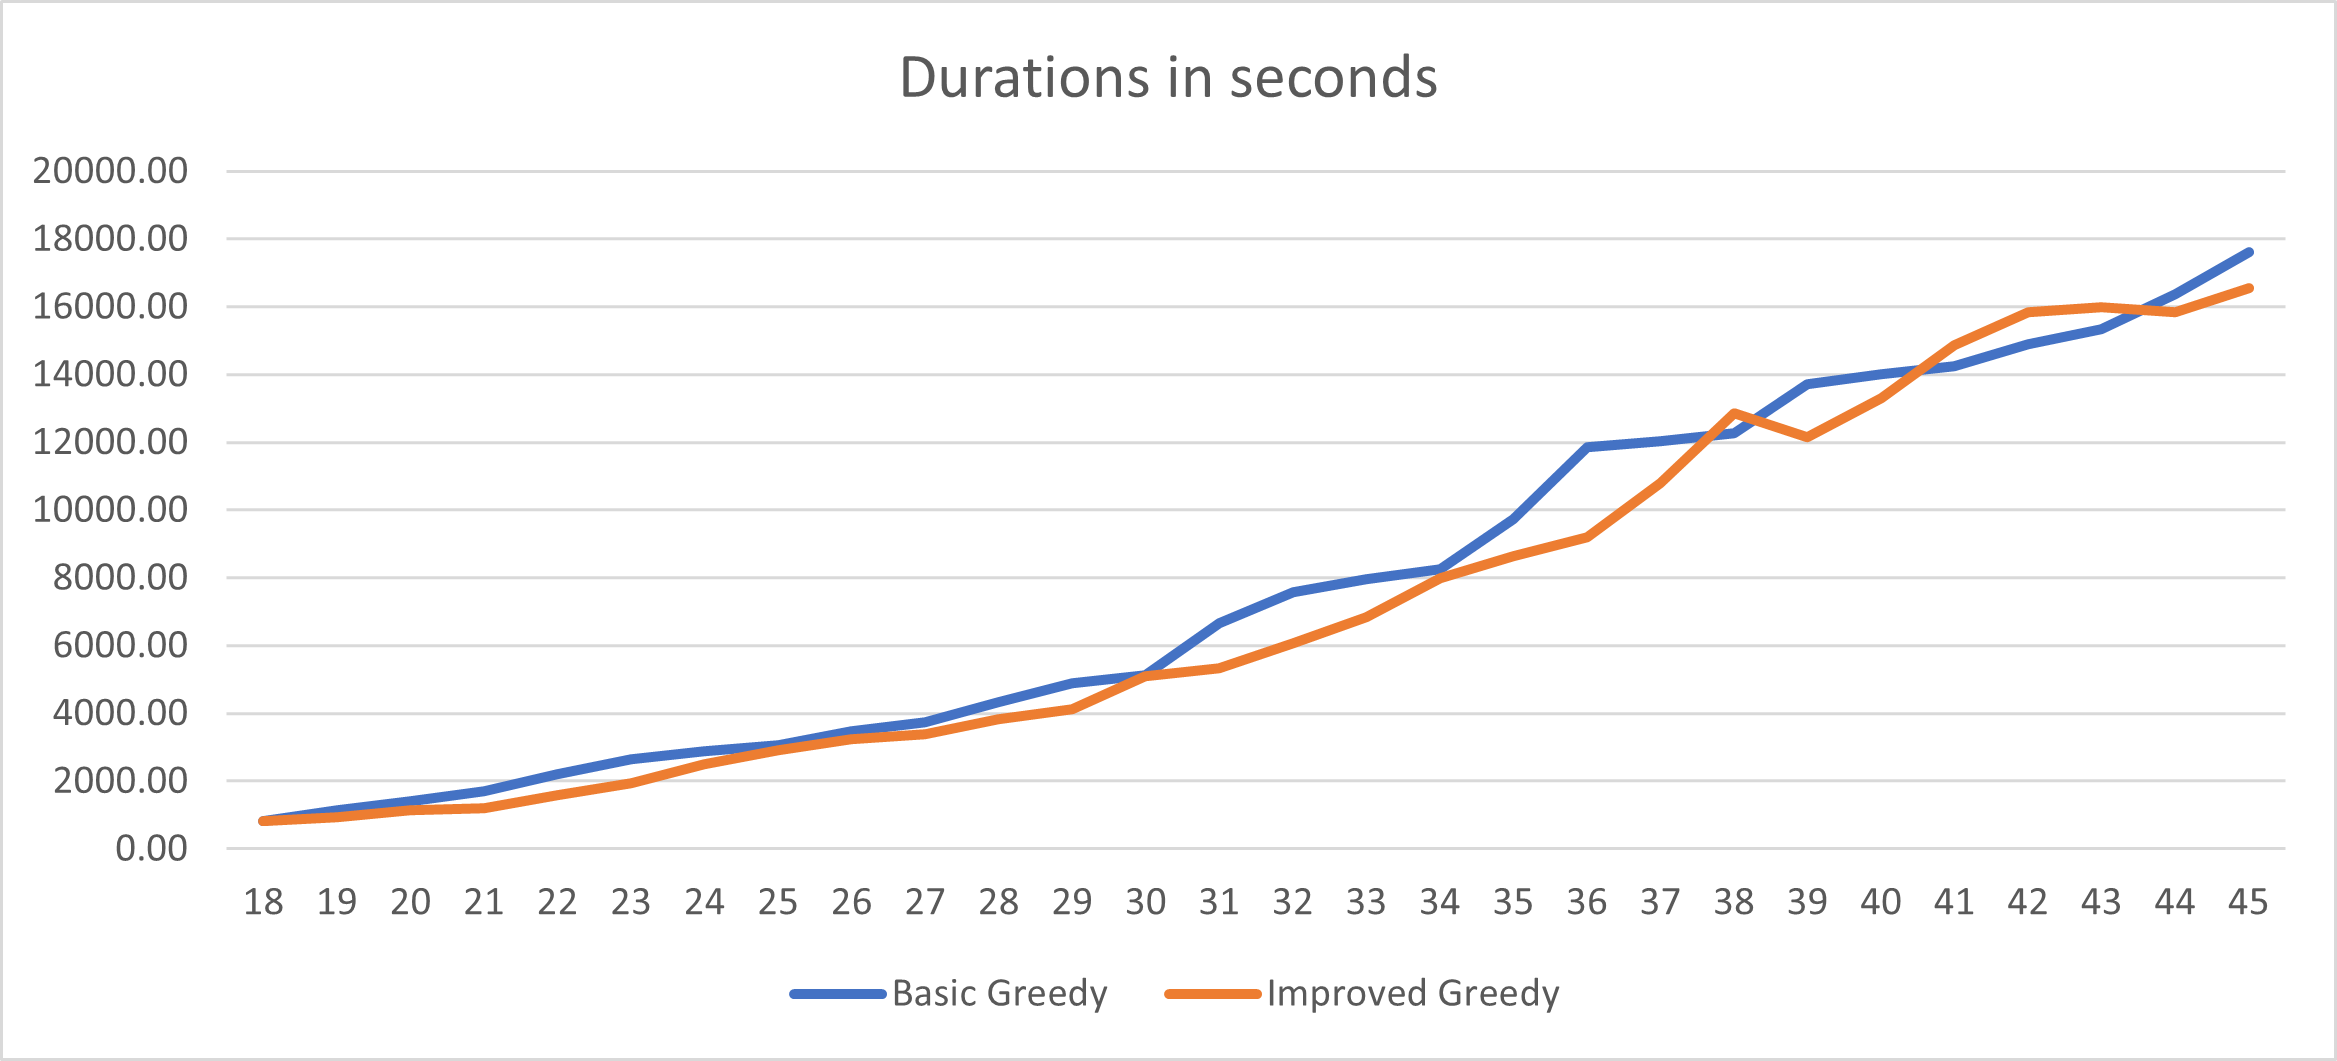
\includegraphics[width=.7\linewidth]{durations_ub_limited_18_45.png}
            \caption{Execution time in secs for Limited Channel Capacity}
            \label{fig:fig_durations_ub_limited_18_45}
        \end{minipage}%
        \begin{minipage}{.6\textwidth}
            \centering
            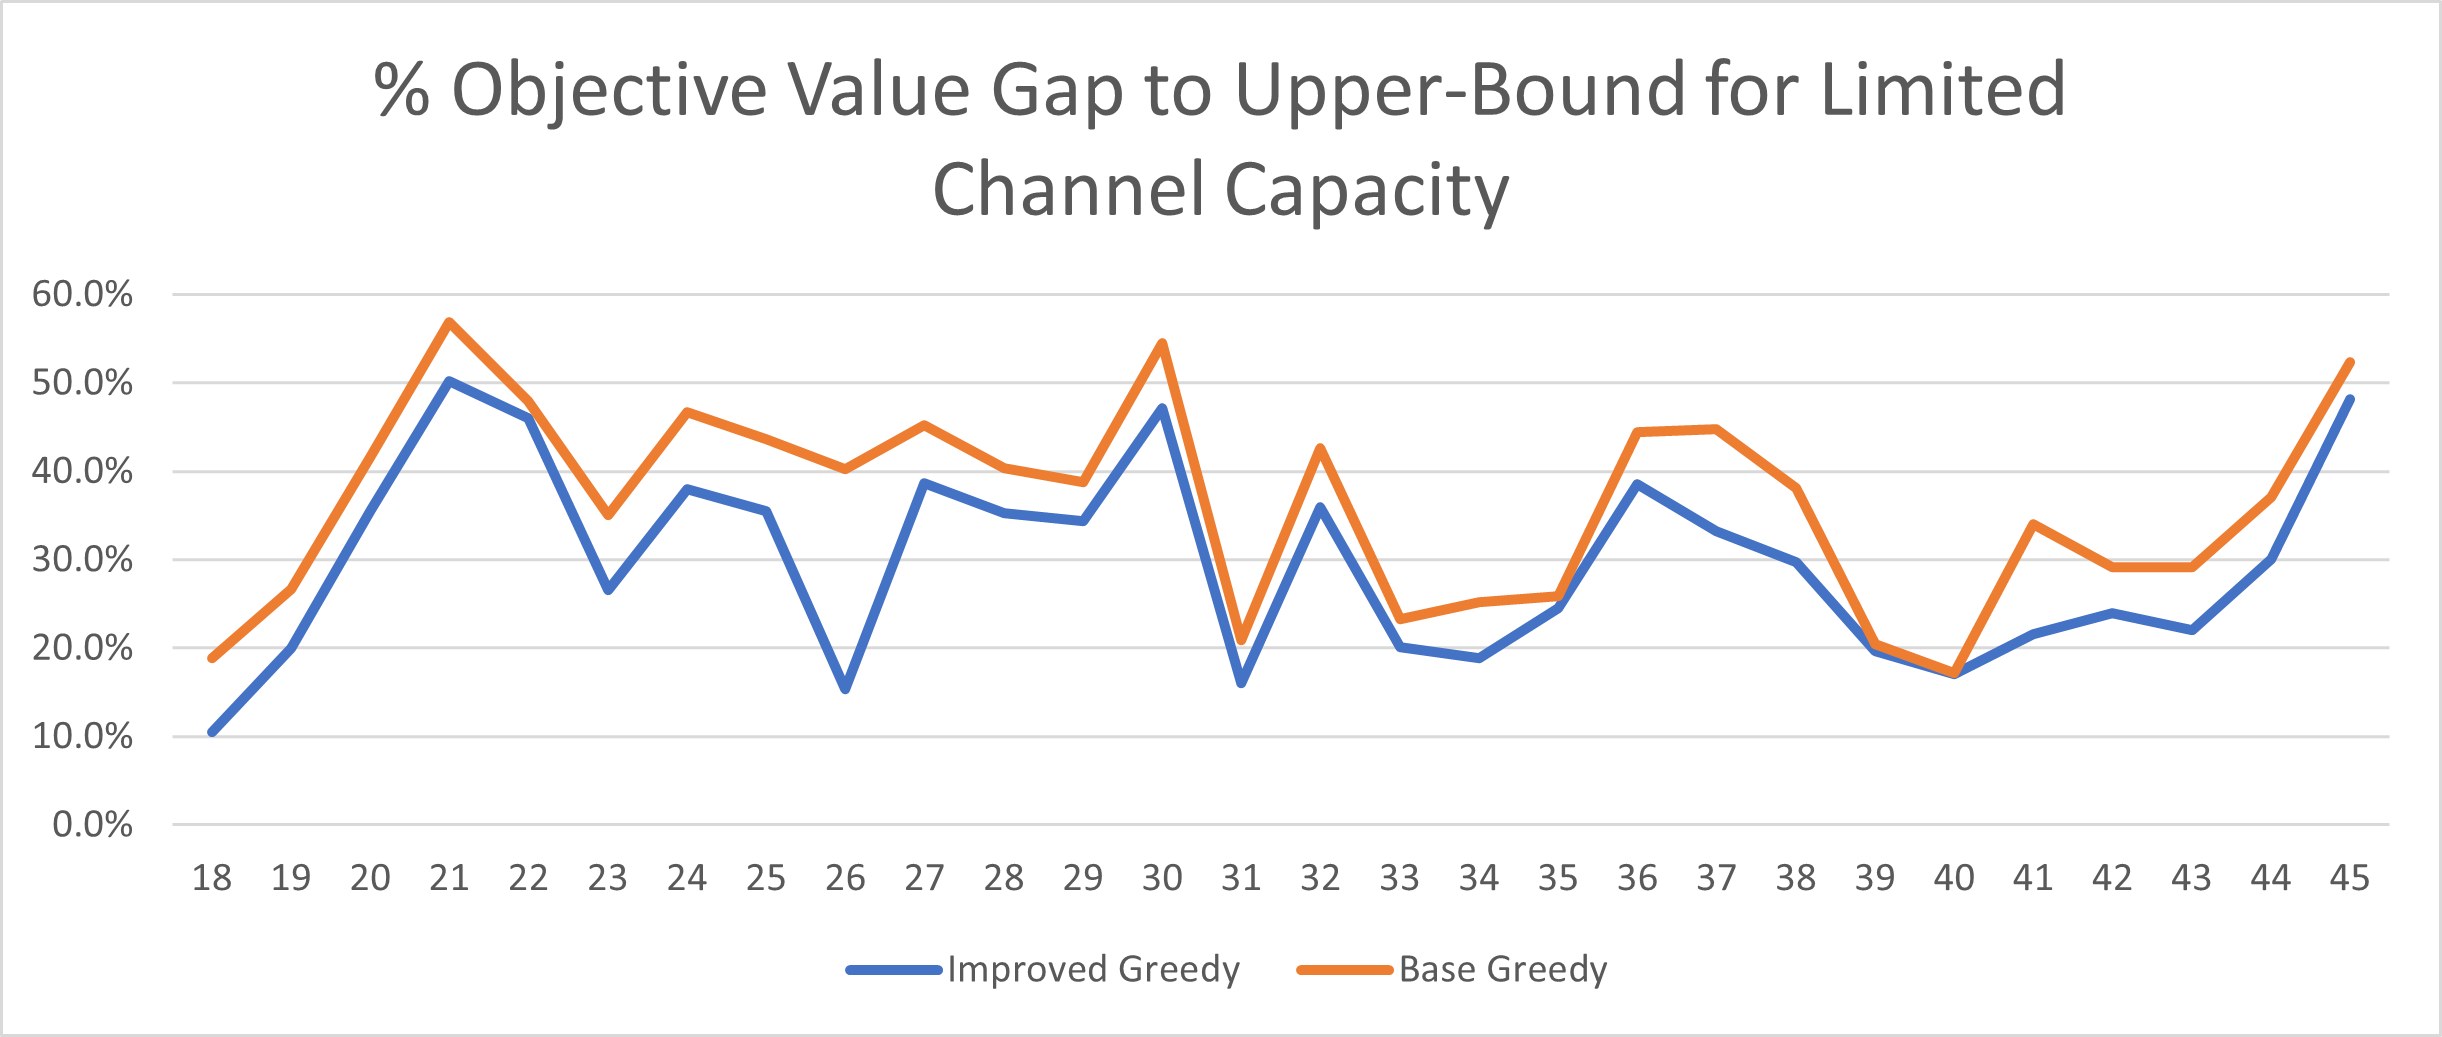
\includegraphics[width=.7\linewidth]{performance_ub_limited_18_45.png}
            \caption{\% Objective Value Gap to Upper-Bound for Limited Channel Capacity}
            \label{fig:fig_value_gap_ub_limited_18_45}
        \end{minipage}
        \end{figure}

        
\newpage
In order to assess the solutions provided by heuristics against the exact solution, we calculate their distance to the exact solution using the formulation described at \equationautorefname \eqref{exact_distance_formulation}, and calculated objective value gaps are presented at table-\ref{table:tbl_17_results}.\\

\noindent $V_{e}$: Exact objective value found by CPLEX-MIP solver. \\
\noindent $V_{h}$: Objective value found by heuristic. \\
\noindent $D_{h}$: Delta of heuristic result regarding exact solution. \\
\begin{align}
&D_{h} = 100 \frac{V_{e} - V_{h}}{V_{e}}, \label{exact_distance_formulation}&
\end{align}\\


During the execution of the model in CPLEX-MIP solution, and CPLEX-LP relaxation heuristics, the memory used increases more than 10GB with a cpu usage of around \%90, while the memory usage were limited to 300MB with a cpu usage around \%20 in both Basis Greedy heuristics, and the LP improved Greedy heuristics.\\

Using first 17 instances we concluded that the Improved Greedy described in \S \ref{s:greedy_heuristic_improved} provides results that are near to exact solution in reasonable execution times, so we tested our next 21 instances (from instace 18 to 38) using only Improved Greedy approach against exact solution. In order find exact solution for instances between 18 and 38, we used parallelization technics. Table-\ref{table:tbl_38_results} presents the objective value gap of Improved Greedy approach for larger test instances.

        \begin{table}[htb!]
        \centering
        \caption{Objective Value Gap\% for Larger Problems}\label{table:tbl_38_results}
       \resizebox{0.65\textwidth}{!}{\begin{minipage}{\textwidth}
        \begin{adjustbox}{max width=1\textwidth}
        \csvautobooktabular{n_test_results_38.csv}
        \end{adjustbox}
        \end{minipage} }
        \end{table}
         \newpage

\section{Conclusion} \label{s:conclusion}
In this study, we discussed a campaign optimization problem, prior to this study literature mostly discussed the problems on finding right target audience, and optimization of it, against cost of delivery and return of investment. In this study our approach is to optimize an existing target audience against communication limitations, both not to irritate customer and be compliant with regulations such as GDPR. We mathematically modeled the problem described at \S \ref{s:problem-model} and later at \S \ref{s:solution-method} offered three heuristic to solve it. A greedy approach that starts with a small LP-model described at \S \ref{s:greedy_heuristic_improved} seems to find good solutions with-in reasonable duration with low memory and cpu.\\
Future research may focus on developing alternative solution methods for the proposed campaign optimization problem. In case of network effect current heuristic can be improved to decrease the gap to the optimal solution. Moreover, new methodologies can be offered to measure the effectiveness of the network.
\newpage

\newpage

\appendix
\section{Appendices}
\subsection{Parameters and Values Used for Test Instancesin case of Rich Channel Capacity}\label{s:apendix-parameters-in-test-instances}
\begin{lstlisting}[language=Python]
Instance - 1
=================================
q_ic:
[[0 1]
 [1 1]
 [0 0]]
rp_c: [62 49]
b: 7
k: 3
l_c: [3 3]
m_i: [4 3 3]
n_i: [3 2 1]
t_hd:
[[70. 70. 60. 50. 50. 70. 70.]
 [70. 60. 70. 60. 50. 60. 70.]
 [50. 60. 60. 50. 50. 60. 50.]]

\end{lstlisting}

\begin{lstlisting}[language=Python]
Instance - 2
=================================
q_ic:
[[0 1 0 1 1]
 [1 0 1 1 0]
 [1 1 1 1 1]]
rp_c: [50 36 40 40 40]
b: 7
k: 3
l_c: [2 4 3 4 2]
m_i: [3 5 3]
n_i: [2 2 3]
t_hd:
[[60. 60. 50. 70. 60. 60. 70.]
 [50. 70. 50. 50. 50. 50. 60.]
 [60. 60. 50. 70. 70. 50. 50.]]

\end{lstlisting}

\begin{lstlisting}[language=Python]
Instance - 3
=================================
q_ic:
[[0 0 0 1 0]
 [0 0 0 0 1]
 [0 0 1 0 1]]
rp_c: [45 61 99 45 45]
b: 7
k: 3
l_c: [3 2 2 2 4]
m_i: [3 5 4]
n_i: [1 1 1]
t_hd:
[[120. 120. 120. 140. 120. 120. 100.]
 [140. 120. 140. 100. 100. 120. 120.]
 [140. 140. 140. 140. 100. 120. 140.]]

\end{lstlisting}

\begin{lstlisting}[language=Python]
Instance - 4
=================================
q_ic:
[[0 0 1 0 1]
 [1 1 1 0 1]
 [1 0 0 0 1]]
rp_c: [22 34 34 34 22]
b: 7
k: 3
l_c: [3 3 3 2 4]
m_i: [3 4 5]
n_i: [2 2 2]
t_hd:
[[300. 250. 300. 250. 350. 250. 300.]
 [250. 250. 350. 250. 300. 300. 250.]
 [250. 250. 300. 300. 300. 300. 300.]]

\end{lstlisting}

\begin{lstlisting}[language=Python]
Instance - 5
=================================
q_ic:
[[1 1 0 0 1]
 [1 1 1 1 0]
 [1 1 1 0 1]]
rp_c: [68 68 68 47 97]
b: 7
k: 3
l_c: [3 2 2 2 3]
m_i: [4 4 4]
n_i: [2 2 2]
t_hd:
[[420. 350. 420. 420. 350. 490. 350.]
 [350. 350. 350. 420. 350. 350. 350.]
 [490. 420. 350. 420. 420. 420. 420.]]

\end{lstlisting}

\begin{lstlisting}[language=Python]
Instance - 6
=================================
q_ic:
[[0 1 1 1 1]
 [1 1 0 1 0]
 [0 1 0 1 0]]
rp_c: [ 7 41  7  7  7]
b: 7
k: 3
l_c: [3 3 4 4 4]
m_i: [3 3 4]
n_i: [2 1 3]
t_hd:
[[700. 700. 600. 600. 500. 600. 500.]
 [500. 500. 600. 500. 700. 600. 500.]
 [500. 700. 500. 500. 500. 500. 600.]]

\end{lstlisting}

\begin{lstlisting}[language=Python]
Instance - 7
=================================
q_ic:
[[1 0 1 0 0 0 0 1 0 0]
 [0 0 1 1 1 0 0 1 1 1]
 [0 0 1 0 1 0 0 0 1 1]]
rp_c: [44 65 45 65 45 45 44 45 45 65]
b: 7
k: 3
l_c: [3 2 2 2 2 3 3 2 2 2]
m_i: [3 3 3]
n_i: [1 1 2]
t_hd:
[[500. 500. 500. 600. 700. 500. 600.]
 [700. 600. 700. 500. 600. 700. 500.]
 [500. 500. 600. 500. 600. 600. 500.]]

\end{lstlisting}

\begin{lstlisting}[language=Python]
Instance - 8
=================================
q_ic:
[[1 0 1 1 0 0 1 1 1 1]
 [0 1 1 1 1 1 1 0 1 1]
 [1 1 0 1 0 0 0 1 0 0]]
rp_c: [66 66 66 66 66 66 66 66 66 21]
b: 7
k: 3
l_c: [4 2 2 4 2 4 4 4 4 4]
m_i: [3 4 4]
n_i: [1 1 2]
t_hd:
[[1000. 1400. 1400. 1200. 1000. 1400. 1000.]
 [1000. 1200. 1000. 1200. 1400. 1200. 1200.]
 [1400. 1400. 1200. 1000. 1200. 1200. 1400.]]

\end{lstlisting}

\begin{lstlisting}[language=Python]
Instance - 9
=================================
q_ic:
[[1 0 1 0 0 1 1 0 1 1]
 [0 1 0 0 0 1 1 1 1 0]
 [0 1 0 1 0 0 0 1 1 1]]
rp_c: [98 42 98 98 42  8  8 98 42 42]
b: 7
k: 3
l_c: [4 3 3 3 4 3 2 3 4 4]
m_i: [4 5 4]
n_i: [1 2 3]
t_hd:
[[2100. 2100. 2100. 2100. 2100. 2100. 1500.]
 [1500. 1800. 1500. 1500. 2100. 1500. 1800.]
 [1500. 2100. 1800. 1800. 2100. 1500. 1500.]]

\end{lstlisting}

\begin{lstlisting}[language=Python]
Instance - 10
=================================
q_ic:
[[0 1 1 1 1 0 1 0 0 1]
 [1 1 0 1 1 0 1 1 1 1]
 [0 0 1 1 0 1 1 1 1 0]]
rp_c: [97 18 18  6 97 18 97  6 97 18]
b: 7
k: 3
l_c: [4 2 4 3 2 3 2 3 2 3]
m_i: [4 3 3]
n_i: [2 2 1]
t_hd:
[[2000. 2000. 2400. 2000. 2800. 2400. 2400.]
 [2400. 2800. 2800. 2000. 2000. 2400. 2000.]
 [2800. 2400. 2000. 2400. 2800. 2800. 2000.]]

\end{lstlisting}

\begin{lstlisting}[language=Python]
Instance - 11
=================================
q_ic:
[[0 1 0 0 0 0 1 1 1 1]
 [0 1 1 1 1 1 0 1 0 0]
 [1 1 0 1 1 0 0 1 0 0]]
rp_c: [69 20 49 49 49 69 69 69 69 20]
b: 7
k: 3
l_c: [2 2 2 3 3 2 3 2 2 4]
m_i: [5 4 3]
n_i: [1 2 1]
t_hd:
[[2500. 2500. 3000. 3500. 2500. 3500. 2500.]
 [2500. 3000. 3500. 3500. 3000. 3500. 3000.]
 [2500. 3000. 3500. 3500. 3000. 3500. 3500.]]

\end{lstlisting}

\begin{lstlisting}[language=Python]
Instance - 12
=================================
q_ic:
[[1 1 0 0 0 1 1 0 0 0]
 [0 1 1 1 1 1 1 1 0 0]
 [0 0 1 0 0 1 1 1 0 1]]
rp_c: [68 62 62 62 68 37 62 62 68 62]
b: 7
k: 3
l_c: [4 2 4 4 2 4 3 3 4 2]
m_i: [5 4 4]
n_i: [2 3 1]
t_hd:
[[5000. 7000. 7000. 5000. 5000. 6000. 5000.]
 [7000. 6000. 5000. 6000. 5000. 5000. 6000.]
 [7000. 5000. 6000. 5000. 6000. 7000. 5000.]]

\end{lstlisting}

\begin{lstlisting}[language=Python]
Instance - 13
=================================
q_ic:
[[1 0 0 0 1 1 1 0 1 0]
 [0 0 0 1 0 0 1 0 1 0]
 [0 0 1 0 0 0 1 1 1 1]]
rp_c: [64 64 38 38 38 80 64 64 64 64]
b: 7
k: 3
l_c: [3 4 2 4 4 3 4 2 4 2]
m_i: [3 5 5]
n_i: [3 1 3]
t_hd:
[[10500. 10500.  7500. 10500.  7500.  9000.  7500.]
 [ 9000.  7500. 10500.  7500.  7500.  9000.  7500.]
 [ 7500. 10500.  7500.  7500.  9000. 10500.  7500.]]

\end{lstlisting}

\begin{lstlisting}[language=Python]
Instance - 14
=================================
q_ic:
[[0 1 0 1 1 1 0 1 1 1]
 [0 1 1 1 1 1 1 1 1 1]
 [0 0 0 1 0 0 1 1 0 1]]
rp_c: [17 29 29 17 56 29 56 56 29 56]
b: 7
k: 3
l_c: [2 2 4 4 4 3 3 2 4 4]
m_i: [5 4 4]
n_i: [3 3 1]
t_hd:
[[14000. 10000. 14000. 10000. 12000. 12000. 12000.]
 [10000. 12000. 14000. 12000. 10000. 10000. 10000.]
 [14000. 10000. 14000. 14000. 10000. 12000. 14000.]]

\end{lstlisting}

\begin{lstlisting}[language=Python]
Instance - 15
=================================
q_ic:
[[1 0 0 1 0 0 1 1 1 0]
 [1 1 1 0 0 0 1 0 0 1]
 [1 1 0 0 1 1 0 1 1 0]]
rp_c: [25 25 25 94 97 97 97 97 94 97]
b: 7
k: 3
l_c: [2 4 2 2 4 2 2 4 4 3]
m_i: [5 4 4]
n_i: [1 1 1]
t_hd:
[[17500. 15000. 12500. 17500. 17500. 15000. 12500.]
 [15000. 15000. 17500. 15000. 12500. 15000. 17500.]
 [17500. 15000. 15000. 12500. 15000. 15000. 15000.]]

\end{lstlisting}

\begin{lstlisting}[language=Python]
Instance - 16
=================================
q_ic:
[[1 1 1 1 0 1 1 0 0 0]
 [0 0 1 0 1 0 0 0 1 1]
 [1 1 1 0 0 1 1 0 1 0]]
rp_c: [17 17 66 66 17 46 66 46 66 66]
b: 7
k: 3
l_c: [2 2 4 2 3 2 3 3 4 3]
m_i: [4 5 3]
n_i: [1 2 1]
t_hd:
[[15000. 21000. 21000. 18000. 21000. 21000. 18000.]
 [18000. 15000. 15000. 18000. 18000. 21000. 18000.]
 [18000. 18000. 18000. 21000. 18000. 15000. 21000.]]

\end{lstlisting}

\begin{lstlisting}[language=Python]
Instance - 17
=================================
q_ic:
[[0 1 0 0 1 1 0 0 1 1]
 [0 1 1 0 1 0 1 1 0 1]
 [0 1 1 1 1 0 1 0 1 0]]
rp_c: [67 48 63 67 67 63 63 63 63 67]
b: 7
k: 3
l_c: [2 4 2 2 2 4 4 2 4 3]
m_i: [5 4 3]
n_i: [2 3 2]
t_hd:
[[21000. 24500. 24500. 24500. 17500. 24500. 24500.]
 [24500. 17500. 21000. 21000. 21000. 17500. 24500.]
 [21000. 17500. 17500. 24500. 21000. 17500. 17500.]]

\end{lstlisting}

\begin{lstlisting}[language=Python]
Instance - 18
=================================
q_ic:
[[1 0 1 1 0 1 1 0 0 1]
 [0 0 1 0 0 1 1 1 0 0]
 [1 0 1 1 1 0 1 0 1 0]]
rp_c: [73 73 73 73 26 58 58 73 73 58]
b: 7
k: 3
l_c: [3 2 3 3 4 3 4 3 3 4]
m_i: [4 5 4]
n_i: [2 2 2]
t_hd:
[[20000. 28000. 28000. 28000. 28000. 24000. 28000.]
 [24000. 20000. 20000. 20000. 28000. 24000. 28000.]
 [28000. 24000. 28000. 20000. 24000. 28000. 24000.]]

\end{lstlisting}

\begin{lstlisting}[language=Python]
Instance - 19
=================================
q_ic:
[[1 1 0 1 0 0 0 0 0 1]
 [0 1 0 1 1 0 0 1 1 0]
 [0 0 0 1 0 1 1 1 0 0]]
rp_c: [40 77 77 40 40 77 40 77 40 16]
b: 7
k: 3
l_c: [2 2 2 4 3 3 4 4 4 3]
m_i: [3 4 3]
n_i: [1 3 2]
t_hd:
[[22500. 22500. 31500. 31500. 27000. 27000. 22500.]
 [27000. 22500. 22500. 31500. 27000. 27000. 22500.]
 [22500. 27000. 22500. 27000. 22500. 27000. 27000.]]

\end{lstlisting}

\begin{lstlisting}[language=Python]
Instance - 20
=================================
q_ic:
[[0 1 0 1 0 1 1 1 1 0]
 [1 0 0 0 0 1 1 1 0 1]
 [0 1 0 0 1 0 1 1 0 1]]
rp_c: [22 22 22 10 52 22 22 22 10 52]
b: 7
k: 3
l_c: [4 2 4 3 3 2 2 4 2 4]
m_i: [5 5 3]
n_i: [3 2 1]
t_hd:
[[30000. 35000. 35000. 30000. 30000. 30000. 30000.]
 [30000. 25000. 25000. 35000. 25000. 35000. 25000.]
 [30000. 25000. 25000. 25000. 35000. 30000. 30000.]]

\end{lstlisting}

\begin{lstlisting}[language=Python]
Instance - 21
=================================
q_ic:
[[1 0 1 0 0 1 1 1 0 0]
 [1 0 1 1 1 0 0 1 0 0]
 [0 0 0 1 0 0 1 0 0 1]]
rp_c: [22 41 21 41 41 41 41 21 21 21]
b: 7
k: 3
l_c: [4 2 3 3 3 2 2 3 3 3]
m_i: [3 5 5]
n_i: [2 2 1]
t_hd:
[[27500. 27500. 27500. 33000. 33000. 27500. 38500.]
 [27500. 33000. 33000. 33000. 38500. 38500. 33000.]
 [38500. 27500. 38500. 33000. 38500. 38500. 38500.]]

\end{lstlisting}

\begin{lstlisting}[language=Python]
Instance - 22
=================================
q_ic:
[[0 0 1 1 1 1 1 0 1 1]
 [1 1 1 0 0 1 1 1 0 1]
 [0 1 0 1 1 0 1 0 0 1]]
rp_c: [49 49 18 18 18 18 36 49 18 18]
b: 7
k: 3
l_c: [4 2 2 4 2 4 2 4 2 2]
m_i: [3 3 4]
n_i: [2 3 3]
t_hd:
[[42000. 42000. 36000. 30000. 30000. 36000. 36000.]
 [36000. 36000. 30000. 30000. 36000. 30000. 30000.]
 [36000. 36000. 42000. 30000. 36000. 42000. 42000.]]

\end{lstlisting}

\begin{lstlisting}[language=Python]
Instance - 23
=================================
q_ic:
[[0 0 1 1 1 0 0 0 0 1]
 [0 0 0 1 1 0 0 1 0 1]
 [1 1 1 1 1 0 1 1 0 1]]
rp_c: [46 20 13 13 20 46 20 20 13 20]
b: 7
k: 3
l_c: [4 2 2 2 2 4 3 2 4 3]
m_i: [3 5 5]
n_i: [2 2 1]
t_hd:
[[45500. 39000. 45500. 32500. 45500. 32500. 45500.]
 [39000. 45500. 45500. 32500. 45500. 39000. 45500.]
 [32500. 45500. 39000. 45500. 39000. 39000. 32500.]]

\end{lstlisting}

\begin{lstlisting}[language=Python]
Instance - 24
=================================
q_ic:
[[0 1 0 0 1 0 1 0 0 0]
 [1 1 1 0 1 0 1 0 1 0]
 [1 1 1 0 1 0 1 0 1 0]]
rp_c: [78 35 80 78 35 78 35 80 78 80]
b: 7
k: 3
l_c: [2 3 3 2 4 3 4 4 2 2]
m_i: [3 5 3]
n_i: [3 3 3]
t_hd:
[[49000. 49000. 49000. 49000. 35000. 42000. 42000.]
 [42000. 49000. 35000. 35000. 42000. 35000. 35000.]
 [42000. 42000. 42000. 35000. 42000. 35000. 49000.]]

\end{lstlisting}

\begin{lstlisting}[language=Python]
Instance - 25
=================================
q_ic:
[[1 0 1 0 0 1 0 1 0 1]
 [0 1 1 1 0 1 0 0 1 1]
 [0 0 0 1 1 1 0 1 0 0]]
rp_c: [66 67  1 67  1 67 67  1  1  1]
b: 7
k: 3
l_c: [4 2 4 2 2 2 2 3 4 3]
m_i: [3 5 3]
n_i: [1 2 3]
t_hd:
[[37500. 37500. 45000. 52500. 37500. 52500. 52500.]
 [37500. 52500. 45000. 52500. 37500. 37500. 52500.]
 [37500. 52500. 37500. 45000. 37500. 45000. 52500.]]

\end{lstlisting}

\begin{lstlisting}[language=Python]
Instance - 26
=================================
q_ic:
[[0 0 1 0 1 0 0 0 0 0]
 [0 0 1 0 0 1 0 0 1 1]
 [0 1 1 0 1 1 1 0 0 1]]
rp_c: [92  0 92  0 92 92 92 92  0 92]
b: 7
k: 3
l_c: [3 2 2 2 2 4 4 3 3 2]
m_i: [5 5 5]
n_i: [3 3 3]
t_hd:
[[56000. 40000. 48000. 40000. 40000. 48000. 56000.]
 [40000. 56000. 48000. 56000. 56000. 48000. 48000.]
 [40000. 48000. 40000. 48000. 48000. 56000. 48000.]]

\end{lstlisting}

\begin{lstlisting}[language=Python]
Instance - 27
=================================
q_ic:
[[1 1 1 0 0 0 1 1 0 1]
 [0 0 0 0 1 0 1 1 0 1]
 [1 1 0 1 1 0 0 0 1 1]]
rp_c: [23 92 23  4 23 92 92 23 23 23]
b: 7
k: 3
l_c: [2 3 3 2 3 2 4 4 4 3]
m_i: [4 4 5]
n_i: [2 1 1]
t_hd:
[[59500. 42500. 51000. 51000. 51000. 42500. 51000.]
 [59500. 42500. 51000. 59500. 51000. 51000. 59500.]
 [51000. 59500. 42500. 42500. 51000. 59500. 42500.]]

\end{lstlisting}

\begin{lstlisting}[language=Python]
Instance - 28
=================================
q_ic:
[[1 0 0 0 0 1 1 0 1 0]
 [1 0 0 0 1 1 1 1 0 1]
 [0 0 0 1 1 0 1 1 1 0]]
rp_c: [71 17 71 45 17 45 17 71 17 17]
b: 7
k: 3
l_c: [4 4 2 2 3 2 4 2 4 4]
m_i: [3 3 5]
n_i: [3 1 1]
t_hd:
[[63000. 45000. 63000. 45000. 54000. 54000. 63000.]
 [63000. 45000. 63000. 63000. 54000. 54000. 54000.]
 [45000. 63000. 54000. 63000. 63000. 54000. 45000.]]

\end{lstlisting}

\begin{lstlisting}[language=Python]
Instance - 29
=================================
q_ic:
[[0 1 0 1 0 0 1 0 1 1]
 [1 1 0 1 1 1 1 0 1 1]
 [1 0 0 0 0 0 1 0 0 1]]
rp_c: [56 14 14 49 56 14 14 14 56 56]
b: 7
k: 3
l_c: [4 3 3 2 3 4 2 4 2 3]
m_i: [4 3 5]
n_i: [2 2 3]
t_hd:
[[66500. 47500. 66500. 57000. 66500. 66500. 47500.]
 [47500. 57000. 57000. 66500. 66500. 57000. 57000.]
 [66500. 47500. 66500. 66500. 47500. 66500. 66500.]]

\end{lstlisting}

\begin{lstlisting}[language=Python]
Instance - 30
=================================
q_ic:
[[1 1 0 1 0 1 1 1 1 1]
 [0 1 1 0 1 1 0 0 1 1]
 [1 1 0 0 0 1 1 1 1 0]]
rp_c: [76 76 33 76 33 33 18 33 18 76]
b: 7
k: 3
l_c: [4 3 2 4 2 2 2 3 2 2]
m_i: [5 5 3]
n_i: [3 2 2]
t_hd:
[[50000. 60000. 60000. 70000. 50000. 60000. 50000.]
 [60000. 70000. 70000. 50000. 50000. 60000. 50000.]
 [50000. 60000. 60000. 70000. 50000. 50000. 60000.]]

\end{lstlisting}

\begin{lstlisting}[language=Python]
Instance - 31
=================================
q_ic:
[[1 1 0 1 0 1 1 1 1 1]
 [0 1 1 0 1 1 0 0 1 1]
 [1 1 0 0 0 1 1 1 1 0]]
rp_c: [76 76 33 76 33 33 18 33 18 76]
b: 7
k: 3
l_c: [4 3 2 4 2 2 2 3 2 2]
m_i: [5 5 3]
n_i: [3 2 2]
t_hd:
[[50000. 60000. 60000. 70000. 50000. 60000. 50000.]
 [60000. 70000. 70000. 50000. 50000. 60000. 50000.]
 [50000. 60000. 60000. 70000. 50000. 50000. 60000.]]

\end{lstlisting}

\begin{lstlisting}[language=Python]
Instance - 32
=================================
q_ic:
[[1 1 0 1 0 0 0 1 0 0]
 [0 0 1 0 0 0 0 0 1 0]
 [1 0 1 0 1 1 1 0 0 1]]
rp_c: [12 24  0 12 12 24 24 24 12  0]
b: 7
k: 3
l_c: [2 3 3 4 2 2 3 2 3 2]
m_i: [3 4 5]
n_i: [2 3 3]
t_hd:
[[ 75000.  75000.  75000.  90000. 105000.  75000.  90000.]
 [ 75000.  90000. 105000.  90000. 105000.  75000.  90000.]
 [ 90000.  90000. 105000.  90000.  75000. 105000. 105000.]]

\end{lstlisting}

\begin{lstlisting}[language=Python]
Instance - 33
=================================
q_ic:
[[1 1 1 0 0 1 1 0 1 1]
 [1 1 1 0 0 0 1 0 1 0]
 [1 1 0 0 1 0 1 0 0 1]]
rp_c: [ 2 83  2  2 42 42 42 83 83  2]
b: 7
k: 3
l_c: [2 4 3 3 2 2 3 3 2 2]
m_i: [4 3 4]
n_i: [1 3 2]
t_hd:
[[100000. 140000. 140000. 120000. 100000. 120000. 100000.]
 [120000. 140000. 120000. 120000. 120000. 120000. 100000.]
 [120000. 140000. 100000. 140000. 120000. 140000. 120000.]]

\end{lstlisting}

\begin{lstlisting}[language=Python]
Instance - 34
=================================
q_ic:
[[1 1 0 1 0 0 1 1 1 0]
 [1 0 1 0 0 0 1 1 1 1]
 [0 1 0 1 0 1 0 1 1 0]]
rp_c: [30 15 15 15 15 15 15 30 83 15]
b: 7
k: 3
l_c: [2 4 4 2 4 3 2 3 4 2]
m_i: [4 3 5]
n_i: [1 1 1]
t_hd:
[[125000. 150000. 150000. 125000. 175000. 125000. 125000.]
 [150000. 175000. 175000. 125000. 150000. 150000. 175000.]
 [175000. 150000. 150000. 175000. 125000. 175000. 150000.]]

\end{lstlisting}

\begin{lstlisting}[language=Python]
Instance - 35
=================================
q_ic:
[[1 0 1 0 1 0 1 0 0 1]
 [1 1 1 1 0 0 0 0 0 1]
 [0 0 1 1 1 0 0 0 0 0]]
rp_c: [43 66 66 43 99 43 43 43 99 66]
b: 7
k: 3
l_c: [4 4 4 2 4 4 2 3 2 4]
m_i: [3 4 5]
n_i: [2 3 2]
t_hd:
[[150000. 210000. 210000. 150000. 180000. 150000. 150000.]
 [210000. 210000. 150000. 180000. 180000. 180000. 210000.]
 [150000. 150000. 180000. 180000. 150000. 210000. 180000.]]

\end{lstlisting}

\begin{lstlisting}[language=Python]
Instance - 36
=================================
q_ic:
[[0 1 0 1 0 1 0 0 1 0]
 [1 0 0 0 1 0 1 1 1 1]
 [1 0 0 0 0 1 0 0 0 1]]
rp_c: [37 37 58 35 35 37 37 58 37 58]
b: 7
k: 3
l_c: [4 4 4 2 2 3 4 2 3 4]
m_i: [5 5 5]
n_i: [3 1 3]
t_hd:
[[245000. 210000. 210000. 210000. 175000. 210000. 245000.]
 [210000. 175000. 175000. 210000. 210000. 245000. 210000.]
 [175000. 245000. 245000. 210000. 175000. 245000. 245000.]]

\end{lstlisting}

\begin{lstlisting}[language=Python]
Instance - 37
=================================
q_ic:
[[1 1 0 0 0 1 0 0 1 0]
 [1 0 1 1 1 1 1 1 1 1]
 [1 0 1 0 1 0 1 1 1 0]]
rp_c: [ 4  4 45  4  4 45 45 63 63 45]
b: 7
k: 3
l_c: [3 3 3 4 2 2 4 4 4 2]
m_i: [4 5 5]
n_i: [1 1 2]
t_hd:
[[280000. 280000. 200000. 240000. 200000. 240000. 240000.]
 [240000. 280000. 280000. 280000. 280000. 280000. 240000.]
 [200000. 240000. 240000. 240000. 280000. 200000. 280000.]]

\end{lstlisting}

\begin{lstlisting}[language=Python]
Instance - 38
=================================
q_ic:
[[1 0 1 0 0 0 1 1 1 1]
 [1 0 1 0 0 1 0 1 1 1]
 [0 1 0 1 1 1 0 1 0 1]]
rp_c: [77 43  2  2 43 43  2 43  2 43]
b: 7
k: 3
l_c: [2 4 3 2 3 3 3 3 2 3]
m_i: [5 5 5]
n_i: [2 3 1]
t_hd:
[[270000. 315000. 270000. 315000. 225000. 270000. 270000.]
 [225000. 315000. 225000. 225000. 315000. 270000. 225000.]
 [225000. 315000. 270000. 270000. 225000. 270000. 225000.]]

\end{lstlisting}

\begin{lstlisting}[language=Python]
Instance - 39
=================================
q_ic:
[[1 1 1 0 0 0 1 0 1 0]
 [0 0 0 1 0 1 1 1 0 0]
 [0 0 1 0 0 1 0 0 1 1]]
rp_c: [21 19 77 77 19 21 19 77 19 77]
b: 7
k: 3
l_c: [3 2 2 4 3 2 3 2 3 2]
m_i: [5 4 3]
n_i: [2 2 2]
t_hd:
[[350000. 250000. 350000. 250000. 300000. 350000. 300000.]
 [250000. 250000. 250000. 350000. 300000. 350000. 350000.]
 [350000. 250000. 350000. 350000. 350000. 300000. 300000.]]

\end{lstlisting}

\begin{lstlisting}[language=Python]
Instance - 40
=================================
q_ic:
[[1 1 0 1 0 1 0 1 0 1]
 [1 0 1 0 0 1 0 1 0 1]
 [0 1 0 0 1 1 1 0 0 1]]
rp_c: [37 60 37 37 60 67 60 67 67 60]
b: 7
k: 3
l_c: [2 2 3 4 3 3 3 2 2 3]
m_i: [3 4 4]
n_i: [2 3 2]
t_hd:
[[330000. 330000. 330000. 275000. 385000. 385000. 330000.]
 [275000. 330000. 330000. 385000. 275000. 385000. 330000.]
 [330000. 385000. 330000. 330000. 385000. 330000. 275000.]]

\end{lstlisting}

\begin{lstlisting}[language=Python]
Instance - 41
=================================
q_ic:
[[0 1 1 0 0 0 0 0 0 1]
 [1 1 1 1 1 1 0 1 1 0]
 [0 1 1 1 1 1 0 1 0 1]]
rp_c: [38 38 38 54 54 54 54 54 92 54]
b: 7
k: 3
l_c: [3 3 4 3 4 3 3 3 3 4]
m_i: [4 5 5]
n_i: [3 2 2]
t_hd:
[[360000. 360000. 360000. 300000. 360000. 420000. 300000.]
 [360000. 420000. 300000. 420000. 420000. 420000. 300000.]
 [360000. 360000. 300000. 420000. 420000. 360000. 420000.]]

\end{lstlisting}

\begin{lstlisting}[language=Python]
Instance - 42
=================================
q_ic:
[[0 0 0 1 0 0 1 0 1 1]
 [1 0 0 0 1 1 0 1 0 1]
 [1 0 0 0 0 1 0 0 1 1]]
rp_c: [42 42 42 76 42 42 71 71 42 71]
b: 7
k: 3
l_c: [2 3 3 3 2 3 4 4 4 3]
m_i: [3 3 4]
n_i: [3 1 3]
t_hd:
[[325000. 325000. 325000. 390000. 455000. 455000. 325000.]
 [325000. 390000. 390000. 390000. 455000. 325000. 390000.]
 [455000. 390000. 455000. 455000. 390000. 390000. 455000.]]

\end{lstlisting}

\begin{lstlisting}[language=Python]
Instance - 43
=================================
q_ic:
[[1 0 0 0 0 1 0 1 0 0]
 [0 1 1 1 0 1 0 1 0 1]
 [0 0 0 0 0 1 1 1 0 0]]
rp_c: [53 53 57 57 53 57 20 20 57 53]
b: 7
k: 3
l_c: [4 2 2 4 2 2 4 4 4 3]
m_i: [4 5 4]
n_i: [1 3 2]
t_hd:
[[350000. 420000. 420000. 490000. 490000. 350000. 420000.]
 [350000. 350000. 420000. 490000. 420000. 350000. 420000.]
 [350000. 350000. 350000. 490000. 490000. 490000. 420000.]]

\end{lstlisting}

\begin{lstlisting}[language=Python]
Instance - 44
=================================
q_ic:
[[0 1 0 1 1 0 1 1 0 0]
 [1 1 0 0 0 1 1 0 0 0]
 [0 1 1 0 1 0 1 1 1 1]]
rp_c: [39 39  2  2 97  2 39 97  2 97]
b: 7
k: 3
l_c: [2 4 2 2 4 2 3 4 3 3]
m_i: [5 3 4]
n_i: [3 1 3]
t_hd:
[[375000. 525000. 450000. 450000. 525000. 525000. 450000.]
 [450000. 525000. 450000. 525000. 450000. 375000. 375000.]
 [525000. 450000. 450000. 450000. 525000. 525000. 450000.]]

\end{lstlisting}

\begin{lstlisting}[language=Python]
Instance - 45
=================================
q_ic:
[[1 0 0 0 1 0 1 1 0 1]
 [0 1 0 1 0 0 1 1 1 1]
 [1 1 0 1 0 0 1 0 1 0]]
rp_c: [32 32 37 37 85 85 32 37 37 32]
b: 7
k: 3
l_c: [3 2 2 3 4 4 4 3 3 3]
m_i: [3 4 4]
n_i: [1 3 3]
t_hd:
[[560000. 560000. 400000. 480000. 560000. 480000. 480000.]
 [480000. 560000. 480000. 560000. 560000. 480000. 560000.]
 [400000. 400000. 560000. 480000. 400000. 400000. 560000.]]

\end{lstlisting}

\subsection{Parameters and Values Used for Test Instances in case of Limited Channel Capacity}\label{s:apendix-parameters-strict-in-test-instances}

\begin{lstlisting}[language=Python]
Instance - 1
=================================
q_ic:
[[0 1]
 [1 1]
 [0 0]]
rp_c: [62 49]
b: 7
k: 3
l_c: [3 3]
m_i: [4 3 3]
n_i: [3 2 1]
t_hd:
[[1. 1. 2. 3. 3. 1. 1.]
 [1. 2. 1. 2. 3. 2. 1.]
 [3. 2. 2. 3. 3. 2. 3.]]

\end{lstlisting}

\begin{lstlisting}[language=Python]
Instance - 2
=================================
q_ic:
[[0 1 0 1 1]
 [1 0 1 1 0]
 [1 1 1 1 1]]
rp_c: [50 36 40 40 40]
b: 7
k: 3
l_c: [2 4 3 4 2]
m_i: [3 5 3]
n_i: [2 2 3]
t_hd:
[[2. 2. 3. 1. 2. 2. 1.]
 [3. 1. 3. 3. 3. 3. 2.]
 [2. 2. 3. 1. 1. 3. 3.]]

\end{lstlisting}

\begin{lstlisting}[language=Python]
Instance - 3
=================================
q_ic:
[[0 0 0 1 0]
 [0 0 0 0 1]
 [0 0 1 0 1]]
rp_c: [45 61 99 45 45]
b: 7
k: 3
l_c: [3 2 2 2 4]
m_i: [3 5 4]
n_i: [1 1 1]
t_hd:
[[4. 4. 4. 2. 4. 4. 6.]
 [2. 4. 2. 6. 6. 4. 4.]
 [2. 2. 2. 2. 6. 4. 2.]]

\end{lstlisting}

\begin{lstlisting}[language=Python]
Instance - 4
=================================
q_ic:
[[0 0 1 0 1]
 [1 1 1 0 1]
 [1 0 0 0 1]]
rp_c: [22 34 34 34 22]
b: 7
k: 3
l_c: [3 3 3 2 4]
m_i: [3 4 5]
n_i: [2 2 2]
t_hd:
[[10. 15. 10. 15.  5. 15. 10.]
 [15. 15.  5. 15. 10. 10. 15.]
 [15. 15. 10. 10. 10. 10. 10.]]

\end{lstlisting}

\begin{lstlisting}[language=Python]
Instance - 5
=================================
q_ic:
[[1 1 0 0 1]
 [1 1 1 1 0]
 [1 1 1 0 1]]
rp_c: [68 68 68 47 97]
b: 7
k: 3
l_c: [3 2 2 2 3]
m_i: [4 4 4]
n_i: [2 2 2]
t_hd:
[[14. 21. 14. 14. 21.  7. 21.]
 [21. 21. 21. 14. 21. 21. 21.]
 [ 7. 14. 21. 14. 14. 14. 14.]]

\end{lstlisting}

\begin{lstlisting}[language=Python]
Instance - 6
=================================
q_ic:
[[0 1 1 1 1]
 [1 1 0 1 0]
 [0 1 0 1 0]]
rp_c: [ 7 41  7  7  7]
b: 7
k: 3
l_c: [3 3 4 4 4]
m_i: [3 3 4]
n_i: [2 1 3]
t_hd:
[[10. 10. 20. 20. 30. 20. 30.]
 [30. 30. 20. 30. 10. 20. 30.]
 [30. 10. 30. 30. 30. 30. 20.]]

\end{lstlisting}

\begin{lstlisting}[language=Python]
Instance - 7
=================================
q_ic:
[[1 0 1 0 0 0 0 1 0 0]
 [0 0 1 1 1 0 0 1 1 1]
 [0 0 1 0 1 0 0 0 1 1]]
rp_c: [44 65 45 65 45 45 44 45 45 65]
b: 7
k: 3
l_c: [3 2 2 2 2 3 3 2 2 2]
m_i: [3 3 3]
n_i: [1 1 2]
t_hd:
[[30. 30. 30. 20. 10. 30. 20.]
 [10. 20. 10. 30. 20. 10. 30.]
 [30. 30. 20. 30. 20. 20. 30.]]

\end{lstlisting}

\begin{lstlisting}[language=Python]
Instance - 8
=================================
q_ic:
[[1 0 1 1 0 0 1 1 1 1]
 [0 1 1 1 1 1 1 0 1 1]
 [1 1 0 1 0 0 0 1 0 0]]
rp_c: [66 66 66 66 66 66 66 66 66 21]
b: 7
k: 3
l_c: [4 2 2 4 2 4 4 4 4 4]
m_i: [3 4 4]
n_i: [1 1 2]
t_hd:
[[60. 20. 20. 40. 60. 20. 60.]
 [60. 40. 60. 40. 20. 40. 40.]
 [20. 20. 40. 60. 40. 40. 20.]]

\end{lstlisting}

\begin{lstlisting}[language=Python]
Instance - 9
=================================
q_ic:
[[1 0 1 0 0 1 1 0 1 1]
 [0 1 0 0 0 1 1 1 1 0]
 [0 1 0 1 0 0 0 1 1 1]]
rp_c: [98 42 98 98 42  8  8 98 42 42]
b: 7
k: 3
l_c: [4 3 3 3 4 3 2 3 4 4]
m_i: [4 5 4]
n_i: [1 2 3]
t_hd:
[[30. 30. 30. 30. 30. 30. 90.]
 [90. 60. 90. 90. 30. 90. 60.]
 [90. 30. 60. 60. 30. 90. 90.]]

\end{lstlisting}

\begin{lstlisting}[language=Python]
Instance - 10
=================================
q_ic:
[[0 1 1 1 1 0 1 0 0 1]
 [1 1 0 1 1 0 1 1 1 1]
 [0 0 1 1 0 1 1 1 1 0]]
rp_c: [97 18 18  6 97 18 97  6 97 18]
b: 7
k: 3
l_c: [4 2 4 3 2 3 2 3 2 3]
m_i: [4 3 3]
n_i: [2 2 1]
t_hd:
[[120. 120.  80. 120.  40.  80.  80.]
 [ 80.  40.  40. 120. 120.  80. 120.]
 [ 40.  80. 120.  80.  40.  40. 120.]]

\end{lstlisting}

\begin{lstlisting}[language=Python]
Instance - 11
=================================
q_ic:
[[0 1 0 0 0 0 1 1 1 1]
 [0 1 1 1 1 1 0 1 0 0]
 [1 1 0 1 1 0 0 1 0 0]]
rp_c: [69 20 49 49 49 69 69 69 69 20]
b: 7
k: 3
l_c: [2 2 2 3 3 2 3 2 2 4]
m_i: [5 4 3]
n_i: [1 2 1]
t_hd:
[[150. 150. 100.  50. 150.  50. 150.]
 [150. 100.  50.  50. 100.  50. 100.]
 [150. 100.  50.  50. 100.  50.  50.]]

\end{lstlisting}

\begin{lstlisting}[language=Python]
Instance - 12
=================================
q_ic:
[[1 1 0 0 0 1 1 0 0 0]
 [0 1 1 1 1 1 1 1 0 0]
 [0 0 1 0 0 1 1 1 0 1]]
rp_c: [68 62 62 62 68 37 62 62 68 62]
b: 7
k: 3
l_c: [4 2 4 4 2 4 3 3 4 2]
m_i: [5 4 4]
n_i: [2 3 1]
t_hd:
[[300. 100. 100. 300. 300. 200. 300.]
 [100. 200. 300. 200. 300. 300. 200.]
 [100. 300. 200. 300. 200. 100. 300.]]

\end{lstlisting}

\begin{lstlisting}[language=Python]
Instance - 13
=================================
q_ic:
[[1 0 0 0 1 1 1 0 1 0]
 [0 0 0 1 0 0 1 0 1 0]
 [0 0 1 0 0 0 1 1 1 1]]
rp_c: [64 64 38 38 38 80 64 64 64 64]
b: 7
k: 3
l_c: [3 4 2 4 4 3 4 2 4 2]
m_i: [3 5 5]
n_i: [3 1 3]
t_hd:
[[150. 150. 450. 150. 450. 300. 450.]
 [300. 450. 150. 450. 450. 300. 450.]
 [450. 150. 450. 450. 300. 150. 450.]]

\end{lstlisting}

\begin{lstlisting}[language=Python]
Instance - 14
=================================
q_ic:
[[0 1 0 1 1 1 0 1 1 1]
 [0 1 1 1 1 1 1 1 1 1]
 [0 0 0 1 0 0 1 1 0 1]]
rp_c: [17 29 29 17 56 29 56 56 29 56]
b: 7
k: 3
l_c: [2 2 4 4 4 3 3 2 4 4]
m_i: [5 4 4]
n_i: [3 3 1]
t_hd:
[[200. 600. 200. 600. 400. 400. 400.]
 [600. 400. 200. 400. 600. 600. 600.]
 [200. 600. 200. 200. 600. 400. 200.]]

\end{lstlisting}

\begin{lstlisting}[language=Python]
Instance - 15
=================================
q_ic:
[[1 0 0 1 0 0 1 1 1 0]
 [1 1 1 0 0 0 1 0 0 1]
 [1 1 0 0 1 1 0 1 1 0]]
rp_c: [25 25 25 94 97 97 97 97 94 97]
b: 7
k: 3
l_c: [2 4 2 2 4 2 2 4 4 3]
m_i: [5 4 4]
n_i: [1 1 1]
t_hd:
[[250. 500. 750. 250. 250. 500. 750.]
 [500. 500. 250. 500. 750. 500. 250.]
 [250. 500. 500. 750. 500. 500. 500.]]

\end{lstlisting}

\begin{lstlisting}[language=Python]
Instance - 16
=================================
q_ic:
[[1 1 1 1 0 1 1 0 0 0]
 [0 0 1 0 1 0 0 0 1 1]
 [1 1 1 0 0 1 1 0 1 0]]
rp_c: [17 17 66 66 17 46 66 46 66 66]
b: 7
k: 3
l_c: [2 2 4 2 3 2 3 3 4 3]
m_i: [4 5 3]
n_i: [1 2 1]
t_hd:
[[900. 300. 300. 600. 300. 300. 600.]
 [600. 900. 900. 600. 600. 300. 600.]
 [600. 600. 600. 300. 600. 900. 300.]]

\end{lstlisting}

\begin{lstlisting}[language=Python]
Instance - 17
=================================
q_ic:
[[0 1 0 0 1 1 0 0 1 1]
 [0 1 1 0 1 0 1 1 0 1]
 [0 1 1 1 1 0 1 0 1 0]]
rp_c: [67 48 63 67 67 63 63 63 63 67]
b: 7
k: 3
l_c: [2 4 2 2 2 4 4 2 4 3]
m_i: [5 4 3]
n_i: [2 3 2]
t_hd:
[[ 700.  350.  350.  350. 1050.  350.  350.]
 [ 350. 1050.  700.  700.  700. 1050.  350.]
 [ 700. 1050. 1050.  350.  700. 1050. 1050.]]

\end{lstlisting}

\begin{lstlisting}[language=Python]
Instance - 18
=================================
q_ic:
[[1 0 1 1 0 1 1 0 0 1]
 [0 0 1 0 0 1 1 1 0 0]
 [1 0 1 1 1 0 1 0 1 0]]
rp_c: [73 73 73 73 26 58 58 73 73 58]
b: 7
k: 3
l_c: [3 2 3 3 4 3 4 3 3 4]
m_i: [4 5 4]
n_i: [2 2 2]
t_hd:
[[1200.  400.  400.  400.  400.  800.  400.]
 [ 800. 1200. 1200. 1200.  400.  800.  400.]
 [ 400.  800.  400. 1200.  800.  400.  800.]]

\end{lstlisting}

\begin{lstlisting}[language=Python]
Instance - 19
=================================
q_ic:
[[1 1 0 1 0 0 0 0 0 1]
 [0 1 0 1 1 0 0 1 1 0]
 [0 0 0 1 0 1 1 1 0 0]]
rp_c: [40 77 77 40 40 77 40 77 40 16]
b: 7
k: 3
l_c: [2 2 2 4 3 3 4 4 4 3]
m_i: [3 4 3]
n_i: [1 3 2]
t_hd:
[[1350. 1350.  450.  450.  900.  900. 1350.]
 [ 900. 1350. 1350.  450.  900.  900. 1350.]
 [1350.  900. 1350.  900. 1350.  900.  900.]]

\end{lstlisting}

\begin{lstlisting}[language=Python]
Instance - 20
=================================
q_ic:
[[0 1 0 1 0 1 1 1 1 0]
 [1 0 0 0 0 1 1 1 0 1]
 [0 1 0 0 1 0 1 1 0 1]]
rp_c: [22 22 22 10 52 22 22 22 10 52]
b: 7
k: 3
l_c: [4 2 4 3 3 2 2 4 2 4]
m_i: [5 5 3]
n_i: [3 2 1]
t_hd:
[[1000.  500.  500. 1000. 1000. 1000. 1000.]
 [1000. 1500. 1500.  500. 1500.  500. 1500.]
 [1000. 1500. 1500. 1500.  500. 1000. 1000.]]

\end{lstlisting}

\begin{lstlisting}[language=Python]
Instance - 21
=================================
q_ic:
[[1 0 1 0 0 1 1 1 0 0]
 [1 0 1 1 1 0 0 1 0 0]
 [0 0 0 1 0 0 1 0 0 1]]
rp_c: [22 41 21 41 41 41 41 21 21 21]
b: 7
k: 3
l_c: [4 2 3 3 3 2 2 3 3 3]
m_i: [3 5 5]
n_i: [2 2 1]
t_hd:
[[1650. 1650. 1650. 1100. 1100. 1650.  550.]
 [1650. 1100. 1100. 1100.  550.  550. 1100.]
 [ 550. 1650.  550. 1100.  550.  550.  550.]]

\end{lstlisting}

\begin{lstlisting}[language=Python]
Instance - 22
=================================
q_ic:
[[0 0 1 1 1 1 1 0 1 1]
 [1 1 1 0 0 1 1 1 0 1]
 [0 1 0 1 1 0 1 0 0 1]]
rp_c: [49 49 18 18 18 18 36 49 18 18]
b: 7
k: 3
l_c: [4 2 2 4 2 4 2 4 2 2]
m_i: [3 3 4]
n_i: [2 3 3]
t_hd:
[[ 600.  600. 1200. 1800. 1800. 1200. 1200.]
 [1200. 1200. 1800. 1800. 1200. 1800. 1800.]
 [1200. 1200.  600. 1800. 1200.  600.  600.]]

\end{lstlisting}

\begin{lstlisting}[language=Python]
Instance - 23
=================================
q_ic:
[[0 0 1 1 1 0 0 0 0 1]
 [0 0 0 1 1 0 0 1 0 1]
 [1 1 1 1 1 0 1 1 0 1]]
rp_c: [46 20 13 13 20 46 20 20 13 20]
b: 7
k: 3
l_c: [4 2 2 2 2 4 3 2 4 3]
m_i: [3 5 5]
n_i: [2 2 1]
t_hd:
[[ 650. 1300.  650. 1950.  650. 1950.  650.]
 [1300.  650.  650. 1950.  650. 1300.  650.]
 [1950.  650. 1300.  650. 1300. 1300. 1950.]]

\end{lstlisting}

\begin{lstlisting}[language=Python]
Instance - 24
=================================
q_ic:
[[0 1 0 0 1 0 1 0 0 0]
 [1 1 1 0 1 0 1 0 1 0]
 [1 1 1 0 1 0 1 0 1 0]]
rp_c: [78 35 80 78 35 78 35 80 78 80]
b: 7
k: 3
l_c: [2 3 3 2 4 3 4 4 2 2]
m_i: [3 5 3]
n_i: [3 3 3]
t_hd:
[[ 700.  700.  700.  700. 2100. 1400. 1400.]
 [1400.  700. 2100. 2100. 1400. 2100. 2100.]
 [1400. 1400. 1400. 2100. 1400. 2100.  700.]]

\end{lstlisting}

\begin{lstlisting}[language=Python]
Instance - 25
=================================
q_ic:
[[1 0 1 0 0 1 0 1 0 1]
 [0 1 1 1 0 1 0 0 1 1]
 [0 0 0 1 1 1 0 1 0 0]]
rp_c: [66 67  1 67  1 67 67  1  1  1]
b: 7
k: 3
l_c: [4 2 4 2 2 2 2 3 4 3]
m_i: [3 5 3]
n_i: [1 2 3]
t_hd:
[[2250. 2250. 1500.  750. 2250.  750.  750.]
 [2250.  750. 1500.  750. 2250. 2250.  750.]
 [2250.  750. 2250. 1500. 2250. 1500.  750.]]

\end{lstlisting}

\begin{lstlisting}[language=Python]
Instance - 26
=================================
q_ic:
[[0 0 1 0 1 0 0 0 0 0]
 [0 0 1 0 0 1 0 0 1 1]
 [0 1 1 0 1 1 1 0 0 1]]
rp_c: [92  0 92  0 92 92 92 92  0 92]
b: 7
k: 3
l_c: [3 2 2 2 2 4 4 3 3 2]
m_i: [5 5 5]
n_i: [3 3 3]
t_hd:
[[ 800. 2400. 1600. 2400. 2400. 1600.  800.]
 [2400.  800. 1600.  800.  800. 1600. 1600.]
 [2400. 1600. 2400. 1600. 1600.  800. 1600.]]

\end{lstlisting}

\begin{lstlisting}[language=Python]
Instance - 27
=================================
q_ic:
[[1 1 1 0 0 0 1 1 0 1]
 [0 0 0 0 1 0 1 1 0 1]
 [1 1 0 1 1 0 0 0 1 1]]
rp_c: [23 92 23  4 23 92 92 23 23 23]
b: 7
k: 3
l_c: [2 3 3 2 3 2 4 4 4 3]
m_i: [4 4 5]
n_i: [2 1 1]
t_hd:
[[ 850. 2550. 1700. 1700. 1700. 2550. 1700.]
 [ 850. 2550. 1700.  850. 1700. 1700.  850.]
 [1700.  850. 2550. 2550. 1700.  850. 2550.]]

\end{lstlisting}

\begin{lstlisting}[language=Python]
Instance - 28
=================================
q_ic:
[[1 0 0 0 0 1 1 0 1 0]
 [1 0 0 0 1 1 1 1 0 1]
 [0 0 0 1 1 0 1 1 1 0]]
rp_c: [71 17 71 45 17 45 17 71 17 17]
b: 7
k: 3
l_c: [4 4 2 2 3 2 4 2 4 4]
m_i: [3 3 5]
n_i: [3 1 1]
t_hd:
[[ 900. 2700.  900. 2700. 1800. 1800.  900.]
 [ 900. 2700.  900.  900. 1800. 1800. 1800.]
 [2700.  900. 1800.  900.  900. 1800. 2700.]]

\end{lstlisting}

\begin{lstlisting}[language=Python]
Instance - 29
=================================
q_ic:
[[0 1 0 1 0 0 1 0 1 1]
 [1 1 0 1 1 1 1 0 1 1]
 [1 0 0 0 0 0 1 0 0 1]]
rp_c: [56 14 14 49 56 14 14 14 56 56]
b: 7
k: 3
l_c: [4 3 3 2 3 4 2 4 2 3]
m_i: [4 3 5]
n_i: [2 2 3]
t_hd:
[[ 950. 2850.  950. 1900.  950.  950. 2850.]
 [2850. 1900. 1900.  950.  950. 1900. 1900.]
 [ 950. 2850.  950.  950. 2850.  950.  950.]]

\end{lstlisting}

\begin{lstlisting}[language=Python]
Instance - 30
=================================
q_ic:
[[1 1 0 1 0 1 1 1 1 1]
 [0 1 1 0 1 1 0 0 1 1]
 [1 1 0 0 0 1 1 1 1 0]]
rp_c: [76 76 33 76 33 33 18 33 18 76]
b: 7
k: 3
l_c: [4 3 2 4 2 2 2 3 2 2]
m_i: [5 5 3]
n_i: [3 2 2]
t_hd:
[[3000. 2000. 2000. 1000. 3000. 2000. 3000.]
 [2000. 1000. 1000. 3000. 3000. 2000. 3000.]
 [3000. 2000. 2000. 1000. 3000. 3000. 2000.]]

\end{lstlisting}

\begin{lstlisting}[language=Python]
Instance - 31
=================================
q_ic:
[[1 1 0 1 0 1 1 1 1 1]
 [0 1 1 0 1 1 0 0 1 1]
 [1 1 0 0 0 1 1 1 1 0]]
rp_c: [76 76 33 76 33 33 18 33 18 76]
b: 7
k: 3
l_c: [4 3 2 4 2 2 2 3 2 2]
m_i: [5 5 3]
n_i: [3 2 2]
t_hd:
[[3000. 2000. 2000. 1000. 3000. 2000. 3000.]
 [2000. 1000. 1000. 3000. 3000. 2000. 3000.]
 [3000. 2000. 2000. 1000. 3000. 3000. 2000.]]

\end{lstlisting}

\begin{lstlisting}[language=Python]
Instance - 32
=================================
q_ic:
[[1 1 0 1 0 0 0 1 0 0]
 [0 0 1 0 0 0 0 0 1 0]
 [1 0 1 0 1 1 1 0 0 1]]
rp_c: [12 24  0 12 12 24 24 24 12  0]
b: 7
k: 3
l_c: [2 3 3 4 2 2 3 2 3 2]
m_i: [3 4 5]
n_i: [2 3 3]
t_hd:
[[4500. 4500. 4500. 3000. 1500. 4500. 3000.]
 [4500. 3000. 1500. 3000. 1500. 4500. 3000.]
 [3000. 3000. 1500. 3000. 4500. 1500. 1500.]]

\end{lstlisting}

\begin{lstlisting}[language=Python]
Instance - 33
=================================
q_ic:
[[1 1 1 0 0 1 1 0 1 1]
 [1 1 1 0 0 0 1 0 1 0]
 [1 1 0 0 1 0 1 0 0 1]]
rp_c: [ 2 83  2  2 42 42 42 83 83  2]
b: 7
k: 3
l_c: [2 4 3 3 2 2 3 3 2 2]
m_i: [4 3 4]
n_i: [1 3 2]
t_hd:
[[6000. 2000. 2000. 4000. 6000. 4000. 6000.]
 [4000. 2000. 4000. 4000. 4000. 4000. 6000.]
 [4000. 2000. 6000. 2000. 4000. 2000. 4000.]]

\end{lstlisting}

\begin{lstlisting}[language=Python]
Instance - 34
=================================
q_ic:
[[1 1 0 1 0 0 1 1 1 0]
 [1 0 1 0 0 0 1 1 1 1]
 [0 1 0 1 0 1 0 1 1 0]]
rp_c: [30 15 15 15 15 15 15 30 83 15]
b: 7
k: 3
l_c: [2 4 4 2 4 3 2 3 4 2]
m_i: [4 3 5]
n_i: [1 1 1]
t_hd:
[[7500. 5000. 5000. 7500. 2500. 7500. 7500.]
 [5000. 2500. 2500. 7500. 5000. 5000. 2500.]
 [2500. 5000. 5000. 2500. 7500. 2500. 5000.]]

\end{lstlisting}

\begin{lstlisting}[language=Python]
Instance - 35
=================================
q_ic:
[[1 0 1 0 1 0 1 0 0 1]
 [1 1 1 1 0 0 0 0 0 1]
 [0 0 1 1 1 0 0 0 0 0]]
rp_c: [43 66 66 43 99 43 43 43 99 66]
b: 7
k: 3
l_c: [4 4 4 2 4 4 2 3 2 4]
m_i: [3 4 5]
n_i: [2 3 2]
t_hd:
[[9000. 3000. 3000. 9000. 6000. 9000. 9000.]
 [3000. 3000. 9000. 6000. 6000. 6000. 3000.]
 [9000. 9000. 6000. 6000. 9000. 3000. 6000.]]

\end{lstlisting}

\begin{lstlisting}[language=Python]
Instance - 36
=================================
q_ic:
[[0 1 0 1 0 1 0 0 1 0]
 [1 0 0 0 1 0 1 1 1 1]
 [1 0 0 0 0 1 0 0 0 1]]
rp_c: [37 37 58 35 35 37 37 58 37 58]
b: 7
k: 3
l_c: [4 4 4 2 2 3 4 2 3 4]
m_i: [5 5 5]
n_i: [3 1 3]
t_hd:
[[ 3500.  7000.  7000.  7000. 10500.  7000.  3500.]
 [ 7000. 10500. 10500.  7000.  7000.  3500.  7000.]
 [10500.  3500.  3500.  7000. 10500.  3500.  3500.]]

\end{lstlisting}

\begin{lstlisting}[language=Python]
Instance - 37
=================================
q_ic:
[[1 1 0 0 0 1 0 0 1 0]
 [1 0 1 1 1 1 1 1 1 1]
 [1 0 1 0 1 0 1 1 1 0]]
rp_c: [ 4  4 45  4  4 45 45 63 63 45]
b: 7
k: 3
l_c: [3 3 3 4 2 2 4 4 4 2]
m_i: [4 5 5]
n_i: [1 1 2]
t_hd:
[[ 4000.  4000. 12000.  8000. 12000.  8000.  8000.]
 [ 8000.  4000.  4000.  4000.  4000.  4000.  8000.]
 [12000.  8000.  8000.  8000.  4000. 12000.  4000.]]

\end{lstlisting}

\begin{lstlisting}[language=Python]
Instance - 38
=================================
q_ic:
[[1 0 1 0 0 0 1 1 1 1]
 [1 0 1 0 0 1 0 1 1 1]
 [0 1 0 1 1 1 0 1 0 1]]
rp_c: [77 43  2  2 43 43  2 43  2 43]
b: 7
k: 3
l_c: [2 4 3 2 3 3 3 3 2 3]
m_i: [5 5 5]
n_i: [2 3 1]
t_hd:
[[ 9000.  4500.  9000.  4500. 13500.  9000.  9000.]
 [13500.  4500. 13500. 13500.  4500.  9000. 13500.]
 [13500.  4500.  9000.  9000. 13500.  9000. 13500.]]

\end{lstlisting}

\begin{lstlisting}[language=Python]
Instance - 39
=================================
q_ic:
[[1 1 1 0 0 0 1 0 1 0]
 [0 0 0 1 0 1 1 1 0 0]
 [0 0 1 0 0 1 0 0 1 1]]
rp_c: [21 19 77 77 19 21 19 77 19 77]
b: 7
k: 3
l_c: [3 2 2 4 3 2 3 2 3 2]
m_i: [5 4 3]
n_i: [2 2 2]
t_hd:
[[ 5000. 15000.  5000. 15000. 10000.  5000. 10000.]
 [15000. 15000. 15000.  5000. 10000.  5000.  5000.]
 [ 5000. 15000.  5000.  5000.  5000. 10000. 10000.]]

\end{lstlisting}

\begin{lstlisting}[language=Python]
Instance - 40
=================================
q_ic:
[[1 1 0 1 0 1 0 1 0 1]
 [1 0 1 0 0 1 0 1 0 1]
 [0 1 0 0 1 1 1 0 0 1]]
rp_c: [37 60 37 37 60 67 60 67 67 60]
b: 7
k: 3
l_c: [2 2 3 4 3 3 3 2 2 3]
m_i: [3 4 4]
n_i: [2 3 2]
t_hd:
[[11000. 11000. 11000. 16500.  5500.  5500. 11000.]
 [16500. 11000. 11000.  5500. 16500.  5500. 11000.]
 [11000.  5500. 11000. 11000.  5500. 11000. 16500.]]

\end{lstlisting}

\begin{lstlisting}[language=Python]
Instance - 41
=================================
q_ic:
[[0 1 1 0 0 0 0 0 0 1]
 [1 1 1 1 1 1 0 1 1 0]
 [0 1 1 1 1 1 0 1 0 1]]
rp_c: [38 38 38 54 54 54 54 54 92 54]
b: 7
k: 3
l_c: [3 3 4 3 4 3 3 3 3 4]
m_i: [4 5 5]
n_i: [3 2 2]
t_hd:
[[12000. 12000. 12000. 18000. 12000.  6000. 18000.]
 [12000.  6000. 18000.  6000.  6000.  6000. 18000.]
 [12000. 12000. 18000.  6000.  6000. 12000.  6000.]]

\end{lstlisting}

\begin{lstlisting}[language=Python]
Instance - 42
=================================
q_ic:
[[0 0 0 1 0 0 1 0 1 1]
 [1 0 0 0 1 1 0 1 0 1]
 [1 0 0 0 0 1 0 0 1 1]]
rp_c: [42 42 42 76 42 42 71 71 42 71]
b: 7
k: 3
l_c: [2 3 3 3 2 3 4 4 4 3]
m_i: [3 3 4]
n_i: [3 1 3]
t_hd:
[[19500. 19500. 19500. 13000.  6500.  6500. 19500.]
 [19500. 13000. 13000. 13000.  6500. 19500. 13000.]
 [ 6500. 13000.  6500.  6500. 13000. 13000.  6500.]]

\end{lstlisting}

\begin{lstlisting}[language=Python]
Instance - 43
=================================
q_ic:
[[1 0 0 0 0 1 0 1 0 0]
 [0 1 1 1 0 1 0 1 0 1]
 [0 0 0 0 0 1 1 1 0 0]]
rp_c: [53 53 57 57 53 57 20 20 57 53]
b: 7
k: 3
l_c: [4 2 2 4 2 2 4 4 4 3]
m_i: [4 5 4]
n_i: [1 3 2]
t_hd:
[[21000. 14000. 14000.  7000.  7000. 21000. 14000.]
 [21000. 21000. 14000.  7000. 14000. 21000. 14000.]
 [21000. 21000. 21000.  7000.  7000.  7000. 14000.]]

\end{lstlisting}

\begin{lstlisting}[language=Python]
Instance - 44
=================================
q_ic:
[[0 1 0 1 1 0 1 1 0 0]
 [1 1 0 0 0 1 1 0 0 0]
 [0 1 1 0 1 0 1 1 1 1]]
rp_c: [39 39  2  2 97  2 39 97  2 97]
b: 7
k: 3
l_c: [2 4 2 2 4 2 3 4 3 3]
m_i: [5 3 4]
n_i: [3 1 3]
t_hd:
[[22500.  7500. 15000. 15000.  7500.  7500. 15000.]
 [15000.  7500. 15000.  7500. 15000. 22500. 22500.]
 [ 7500. 15000. 15000. 15000.  7500.  7500. 15000.]]

\end{lstlisting}

\begin{lstlisting}[language=Python]
Instance - 45
=================================
q_ic:
[[1 0 0 0 1 0 1 1 0 1]
 [0 1 0 1 0 0 1 1 1 1]
 [1 1 0 1 0 0 1 0 1 0]]
rp_c: [32 32 37 37 85 85 32 37 37 32]
b: 7
k: 3
l_c: [3 2 2 3 4 4 4 3 3 3]
m_i: [3 4 4]
n_i: [1 3 3]
t_hd:
[[ 8000.  8000. 24000. 16000.  8000. 16000. 16000.]
 [16000.  8000. 16000.  8000.  8000. 16000.  8000.]
 [24000. 24000.  8000. 16000. 24000. 24000.  8000.]]

\end{lstlisting}
\bibliographystyle{chicago}

\bibliography{references}

\end{document}